\chapter{Electrophysiology of Neurons}

\section{Experimental techniques}

The very first step to understand the neuron is to know its morphology.
To determine the shape of neuron, you have to stain it somehow.  There are
several way to do it (Sect.\ref{sec:stain-neuron}).



\subsection{stain the neurons}
\label{sec:stain-neuron}

The brain of the mice is cut at 3 conventional directions: frontal, horizontal,
and sagittal (Sect.\ref{sec:brain-anatomy}.


\subsection{-- Nissl staining (cell's body)}
\label{sec:Nissl-stain}

One of the earliest techniques to allow for the visualization of neurons is the
Nissl Stain.
The Nissl stain reacts with most of the cells in a brain slice (both neurons and
glial cells), so it is not great for seeing the detailed morphology of a single neuron.
However, it is great for 
\begin{itemize}
  \item  seeing the cellular patterns of a particular brain
area. 

  \item used as a control experiment to confirm that a treatment did not kill
  cells or damage the brain.  
  
  \item  visualize the results of a certain mutation or drug treatment on the
  brain. 
\end{itemize}


The Nissl stain colors the cell (purple if you are using cresyl violet on
paraffin or frozen sections) because it reacts with nucleic acids (which make up
DNA and RNA) in the nucleus of the cell and in the endoplasmic reticulum. So, it
typically shows the cell's body.


\subsection{-- Golgi staining}
\label{sec:Golgi-stain}

The Golgi stain works by starting a silver chromate reaction in random cells.
It is not known why a certain cell would undergo the reaction while a cell right
next to it would not. The result is that the morphology of the cells can be
clearly seen without contamination from nearby dendrites from other cells.


This technique can be used   
\begin{itemize}
  \item to test whether a mutation or drug treatment alters the growth of cell
  dendrites.
  
Ref: 
  \url{http://cellularscale.blogspot.com/2012/03/seeing-cells-nissl-and-golgi-together.html}
\end{itemize}


\subsection{-- byocitin filling method}
\label{sec:byocitin-filling}

The biocytin filling method makes use of the same patch clamp electrode to
record the electrical activity of the neuron and to fill it with the biocytin
molecule that can be later dyed.  So this method is perfect for building a
neuron because with it you can correlate the shape of the neuron directly with
its activity patterns \citep{marx2002}.

Basic protocols
\begin{verbatim}
1. make brain slices
2. fill the neuron with biocytin while recording its electrical activity
3. fix the brain slice in paraformaldehyde
4. quench the endogenous peroxidase
5. connect the biocytin to avidin (using the vectastain ABC kit)
6. colorize the avidin (using DAB and nickel)
7. mount the slices on gelatin subbed slides
8. dehydrate the slices SLOWLY through very small steps of ethanol concentration
 (SLOWLY is important to get better morphology)
9. clear with xylene and coverslip
\end{verbatim}


\subsection{build the morphology}

Chap.\ref{chap:neuron-morphology} describes in details.

\subsection{visual dendritic recording technique}
\label{sec:visual-dendritic-recording}

Visual dendritic recording techniques were first made available in 1993-1994
(Stuart et al. 1993; Denk et al. 1994) to study neuron's electrophysiological
behavior at non-somatic regions, e.g. regions on the denrite. 
Good references include:
\begin{enumerate}
  \item pyramidal neuron: larkum-zhu-sakmann (2001)
  
  \item medium-sized spiny neuron (MSN): 
\end{enumerate}

\subsection{cell extraction}

If the data is recorded from {\bf acutely isolated cells} rather than
whole-cell, i.e. there can be loss of currents attributable to the removal of
the dendrites during preparation.




\section{Introduction}

Early views of electrophysiology of mammalian neurons were strongly influenced
by the set of experiment in motoneurons by~\citep{coombs1956tcmr}. An important
aspect is to understand the morphology of neurons (Sect.\ref{sec:stain-neuron}).
Today, thanks to the advances in single-channel recording, and cultured nerve
cells..., there has been a fundamental change in our thinking regarding the
electrical properties of mammalian neurons. However, understanding the channel
distribution along the dendrites, and the electrophysiological properties at
these regions are still challenging. Sect.\ref{sec:visual-dendritic-recording}
describes how experimental methods are being used to help us understanding the
neuron better at a more detailed level.

\subsection{Timelines in history}
\label{sec:timelines}

Until mid 1970s, our understanding of ion channels was limited to the
study of population analysis, i.e. we inhibit all ionic channels,
except for one type and then study the average behavior of the
population containing channels of a single type.

In 1976, {\bf patch-clamp} technique developed by Neher and Sakmann
(Sect.\ref{sec:patch-clamp}) allowed us to record the current flowing across a
single channel. Then, molecular cloning technique allowed us to study the
structure of ion channels.  Patch-clamp technique revealed that ion channels
open and closed randomly. This means that the behavior of ion channels cannot be
predicted and describe by deterministic mathematical equations.

Visual dendritic recording techniques
(Sect.\ref{sec:visual-dendritic-recording}) developed in early 1990s enabled us
to study electrophysiological properties at different regions on the dendritic
tree.

% We will study these in another book, Computational Biology.

\subsection{Ion concentrations}
\label{sec:ion-concentration-neuron}


Resting membrane potential is discussed in
Sect.\ref{sec:resting-membrane-potential}.
The reversal potentials are discussed in Sect.\ref{sec:reversal-potential}.

The intracellular of sodium in neurons, e.g. cultured striatal neuron, is about
15-16 mM; which is considerably higher than that in non-neuronal cells (3-7 mM).
This high $[\Na]_i$ in neurons is attributed to the presence of neuron-specific
catalytic subunit of sodium pump, $\alpha_3$ (Sect.\ref{sec:NaK-isoforms}). Most
non-neuronal cells express only the more widespread $\alpha_1$ isoform.

In a typical nerve cell, the concentration of different ions 
and the resting potential are
given below or in Fig.\ref{fig:ion-concentration}
\begin{verbatim}
        Inside       Outside          Ratio Co/Ci
[Na]    15 mM         145 mM             9.7
[K]     150 mM         5  mM             0.03
[Cl-]   9  mM         125 mM            13.9
[Misc-] 156mM          30 mM             0.2
[Misc+]                 5 mM
[Ca]                  0.85-1.18 mM                (cerebral cortex of cat sleep)
     Vi = -70 mV      Vo = 0mV                   
\end{verbatim}
In the cerebral cortex of the cat during slow wave sleep, $[\Ca]_e$ levels
have been reported to oscillate between 1.18 and 0.85 mM.\citep{amzica2002}.

\ce{Ca^2+} is maintained in outer environment 1000 times higher than
inside, \ce{Na+} is maintained a high concentration outside (about 10 times
compared with inside) while \ce{K+} is maintained a high concentration on the
inside (about 20 times compared with outside).

In addition, the negative charged proteins stay inside of the cell while
the negative \ce{Cl-} stay outside of the cell, as shown in
Fig.\ref{fig:ion-concentration}. 
 
\begin{figure}[htb]
  \centerline{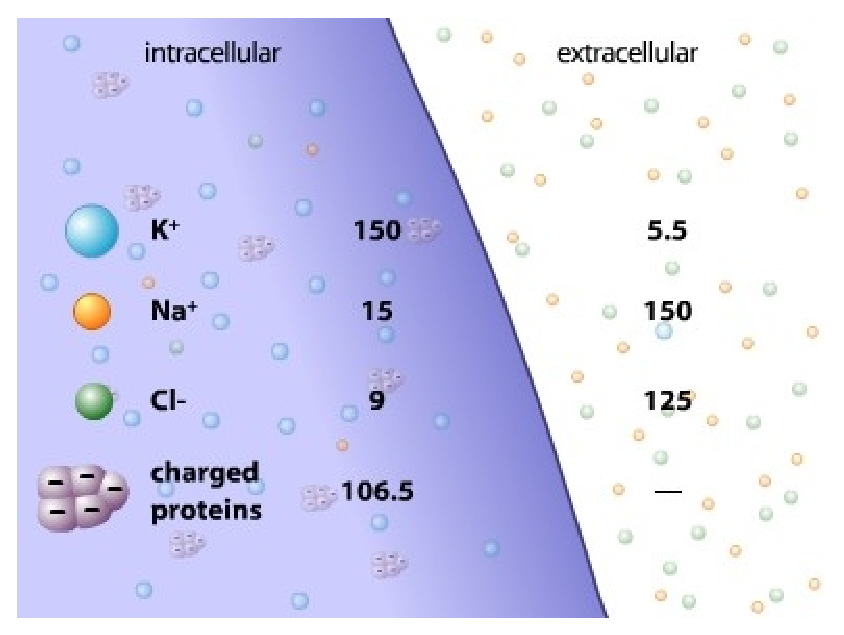
\includegraphics[height=6cm]{./images/ions-concentration.eps}}
  \caption{Ion concentration}\label{fig:ion-concentration}
\end{figure}



\subsection{Rheobase [miliampere, mA] and chronaxie (milisecond, ms)}
\label{sec:rheobase}

Neuronal tissues can be excited by electrical stimulation. Two commonly
encountered characteristics for electrically stimulating nerve cells is the
threshold and the rheobase.

The {\bf threshold} is a measure of membrane excitability, which is the minimal
energy (typically current level and not voltage) applied for a certain duration
to excite neural tissue.

Rheobase is an example of threshold, when the duration is infinite,
Fig.\ref{fig:rheobase}(A).
In neuroscience, {\bf rheobase} (unit: mA) is the {\it minimal current amplitude
of infinite duration} (in a practical sense, about {\it 300 milliseconds}) that
results in the depolarization threshold of the cell membranes being reached,
such as an action potential (Sect.\ref{sec:AP-neuron}) or the contraction of a
muscle.

\begin{figure}[hbt]
  \centerline{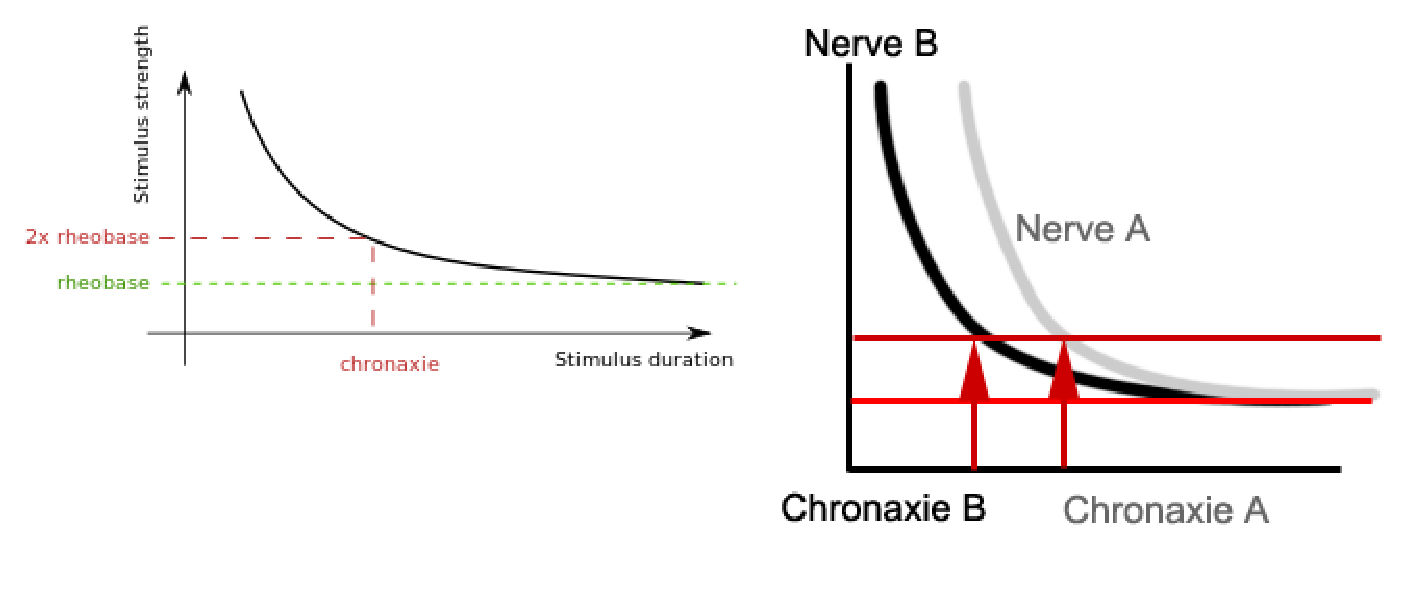
\includegraphics[height=5cm,
    angle=0]{./images/rheobase-chronaxie.eps}}
 \caption{Rheobase (the horizontal asymptote); (B) Chronaxie is the time
 corresponding to the duration required for triggering the excitation upon 2x
 the strength of stimulus}
\label{fig:rheobase}
\end{figure}

If the stimulus is double of the rheobase value, then the pulse duration
required for the excitation is called {\bf Chronaxie}.
When two neurons having the same rheobase, by using chronaxie, it gives an
indication of their relative excitabilities.  In the strength-duration curve to
the right, nerve B is the more excitable, Fig.\ref{fig:rheobase}(B).

\begin{mdframed}
The action potential threshold can be measured in many ways. Using ramp current
or using a series of current steps.

{\bf Series of current steps}: use 10 ms long depolarizing current steps and
pick the action potential fired by the minimum injected current amplitude. 
\end{mdframed}

The function of the strength-duration relationship can be fitted with
a decaying exponential:
\def\rh{{\text{rh}}} 
\def\sd{{\text{sd}}}
\begin{equation}
I = \frac{I_\rh}{\left( 1- \exp(-t/\tau_\sd) \right)}
\end{equation}
with $I$= threshold current-level, $I_\rh$ = rheobase, $t$= stimulus duration,
$\tau_\sd$ = time-constant of the exponential (which is indeed $\tau_\sd=RC$
the membrane time constant).

\url{http://www.medicine.mcgill.ca/physio/vlab/cap/s-d.htm}

\subsection{Conduction velocity}
\label{sec:conduction-velocity}

The conduction velocity of nerve is normally reported in meters per second.  It
is more easily recorded as millimeters per millisecond, which yields the same
result.

In neurons, conduction velocity is systematically related to fibre diameter in
fibres of a given type.
\begin{equation}
\text{velocity (m/s) = diameter} (\mum) \times 2.5
\end{equation}

\subsection{Saltatory conduction}
\label{sec:saltatory-conduction}

Once the AP is triggered on the neuron's soma, the
voltage vonduction slowly on one part of the axon, then very fast at the
myelinated-sheath region, then slow, then very fast again at another
myelinated-sheath region, and so on. 

This conduction behavior, like jumping, is called {\bf saltatory conduction}.

\subsection{Neuron graded potential}

\subsection{Up and Down state of subthreshold membrane potential}
\label{sec:Up-state-resting-potential}
\label{sec:Down-state-resting-potential}

The membrane potential of most neurons have been found to be at two preferred
subthreshold values, i.e. both subthreshold for action potential generation
\footnote{\url{http://www.scholarpedia.org/article/Up_and_down_states}}
As shown in Fig.\ref{fig:Vm-neuron-Up-Down-state}, both cells toggle between two
preferred membrane potentials, one very hyperpolarized (Down state), and one
more depolarized (Up state). In both cells, the Up state is only a few
millivolts from the action potential threshold.
\textcolor{red}{ Neurons may exhibit two-state behavior because of their
intrinsic properties, or because they are in a network that imposes it on them,
or both, and may be expressed as a part of a variety of activity states.}
\begin{itemize}
  
  \item In both the cerebral cortex and the striatum, the {\it Down state} for
  individual neurons is {\bf stable}, and is close to the resting membrane
  potential observed when all input is removed (Wilson et al., 1983b; Timofeev et al.,
  2001)
  
  How about Up state, is it stable?
  
  \item It is well known that some neurons are bistable, meaning that they
  simultaneously possess stable depolarized, as well as hyperpolarized states
  and once placed in either state will remain there with no additional
  stimululation.
  
 Experiment: An appropriate test for stability of the Up state is experimental
 depolarization of the membrane by current injection at a time when the cell
 would otherwise be in the Down state. When the current is released, a bistable
 neuron would remain in the Up state until perturbed again. Lingering in the Up
 state, followed by a return to the Down state after a significant delay, would
 be indicative of the operation of a transiently stable Up state.
 
  \item 
\end{itemize}

 \begin{figure}[htb]
\centerline{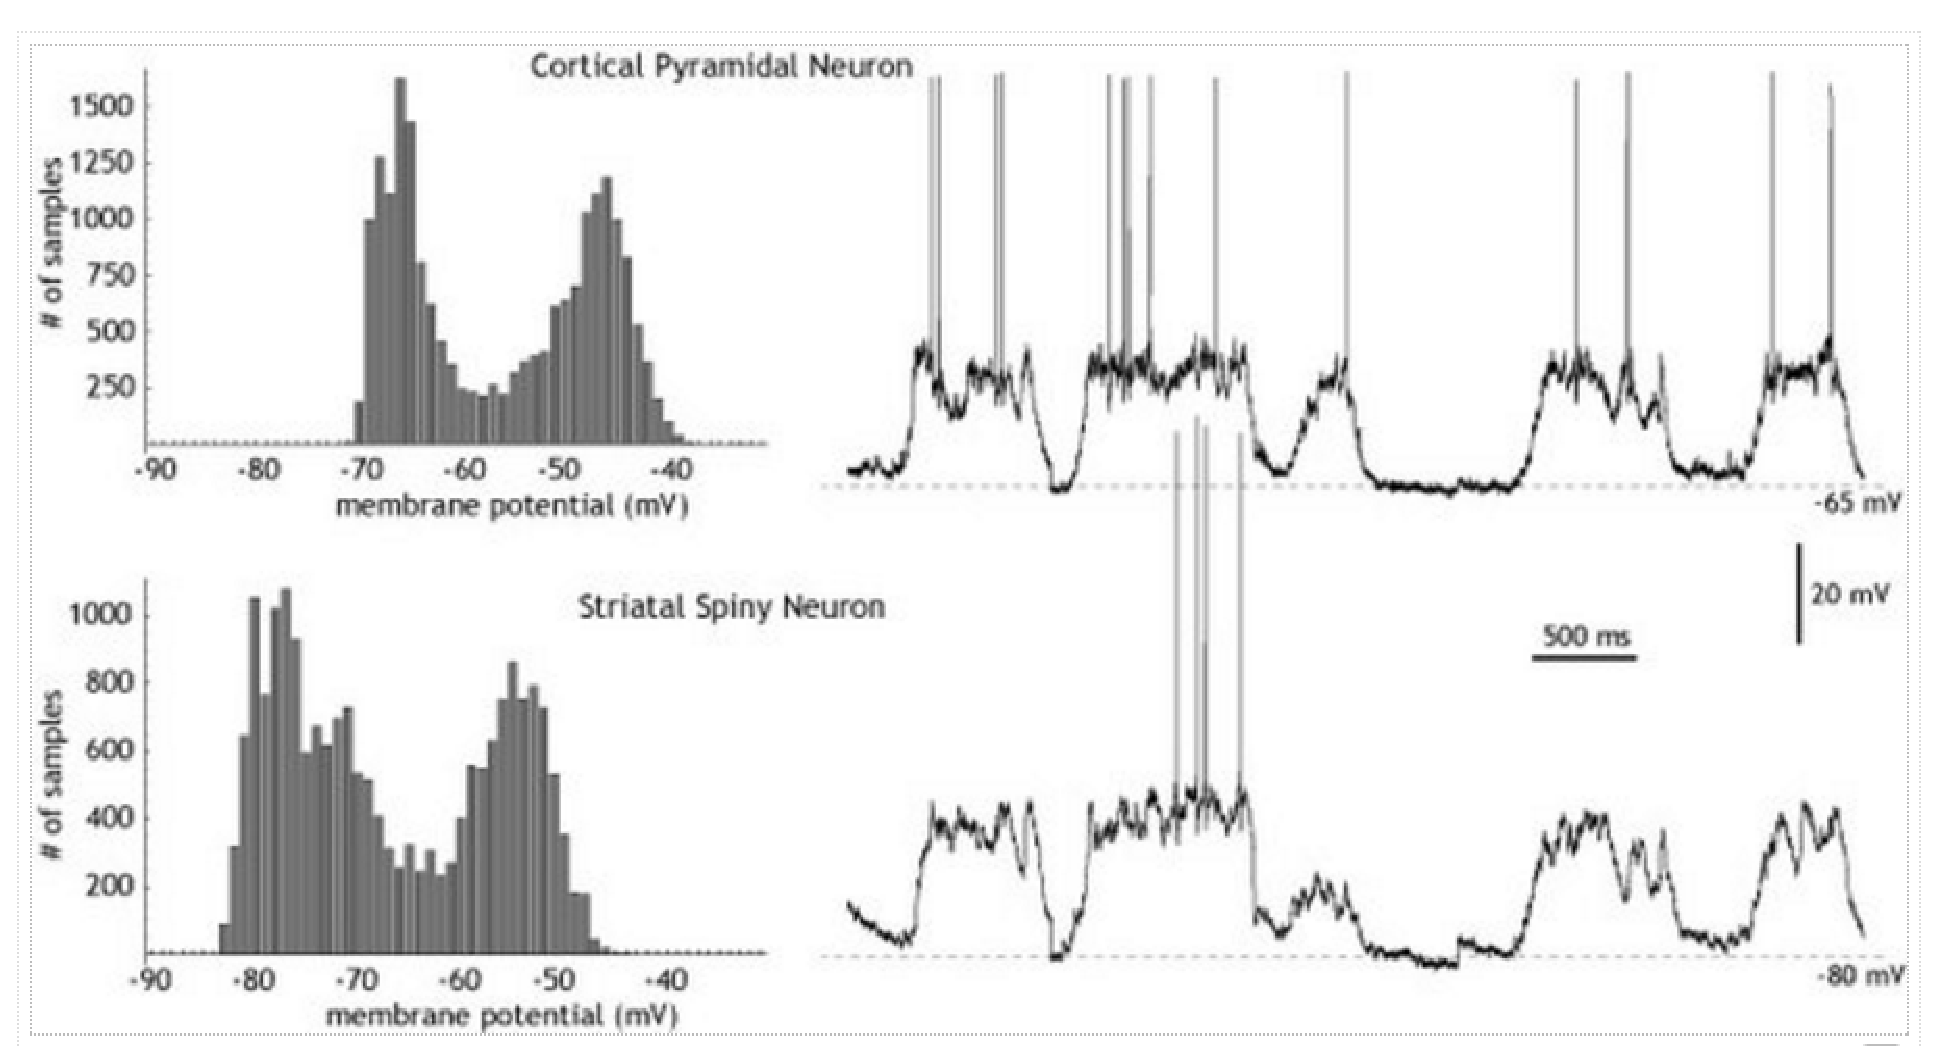
\includegraphics[height=4cm]{./images/Vm-neuron-Up-Down-state.eps}}
\caption{All-points histogram showing
frequency of occurrence of various values of
Vm: upper plots showing for a layer V
pyramidal neuron, and lower plots showing
for a typical striatal projection neuron,
recorded simultaneously}\label{fig:Vm-neuron-Up-Down-state}
\end{figure} 


The stabiliity of the Down state is apparent from examination of the
current-voltage (I-V) curve for the spiny neuron
(Sect.\ref{sec:I-V-curve-inward-rectification}). At membrane potentials
associated with the Down state, the I-V curve slope (the input conductance)
increases with hyperpolarization. This is called inward rectification, or
anomalous rectification (anomalous because it isn't predicted by the
Goldman-Hodgkin-Katz equation).

\begin{itemize}
  \item   In the Down state, the input resistance of the spiny neuron is low
  (10-30 MOhms), making the cell relatively insensitive to small synaptic inputs.
  
  \item The origin of inward rectification in the spiny neuron is a
  hyperpolarization-activated potassium channel, KIR2 (Nisenbaum and Wilson,
  1995) - Sect.\ref{sec:Kir2.x}
\end{itemize}

\subsection{Discharge frequency}
\label{sec:discharge-frequency}

{\bf Discharge} means the neuron fire spontaneously.
Cortical neurons discharge spontaneously in vivo, contributing
to irregular background synaptic inputs to other cells (Shadlen
and Newsome, 1994). This is part of the so-called homeostatic plasticity
(Sect.\ref{sec:homeostatic-plasticity})

The discharge frequency of neurons is affected by their afferents and intrinsic
properties, and shows great individual variability.
Information in neuronal networks is thought to be represented by the rate of
discharge and the temporal relationship between the discharging neurons.
The discharge from presynaptic neuron induces fluctuations in the postsynaptic
membrane voltage (Pare et al., 1998) and strongly affects the neuronal frequency
versus current ( f-I) relationship and input integration (Destexhe et al.,
2003).

However, it remains unclear whether irregular firing and membrane fluctuations
encode relevant information and take active part in signal processing, and
whether a neuron can propagate such information to downstream
neurons.\citep{arsiero2007}.

In the hippocampus, population synchrony fluctuates during theta and gamma
oscillations (10-100 ms scale) and can increase almost 10-fold during sharp wave
bursts. Despite these large changes in excitability in the sub-second scale,
longer-term (minute-scale) firing rates of individual neurons are relatively
constant in an unchanging environment, i.e. mean hippocampal output remains
stable over time. 


\subsection{Action Potential (AP) in nerve cells (spike or burst)}
\label{sec:AP-neuron}

Sect.\ref{sec:AP-cardiac} discusses the AP in myocytes.
The neuron is composed of multiple component (apical dendrite, basal dendrite,
axon, soma), and there are different places where the potential changes can
occurs (spine, dendritic shaft, soma, axon), Fig.\ref{fig:neuron-input-output}.

An AP initiate site is the site at which the membrane potential first pass the
threshold of Na+ spike. In the classic view of synaptic integration, the
synaptic inputs, which cause a small amount of membrane depolarization which
then propagate toward the soma. The spatial and temporal effect of a certain
number of synaptic inputs, then can cause a certain amount of depolarization at
all locations along the dendrites, soma, and AIS; but the region that first pass
the threshold is called the {\bf initiation site}. This is typically the site
with lowest threshold, which can be explained by either
\begin{enumerate}
  \item very high density of Na+ channel, so the activation is likely to trigger
  quicker and more depolarization.
  
  \item the different subtypes of Na+ channel; in that the subtype in that area
  has a lower half activation potential, and is thus more easily activated.
  
  \item the high HCN channel (in some neuron), that bring the resting membrane
  potential there is more depolarized than other regions, and is thus closer to
  the threshold
\end{enumerate}

Once the membrane potential of the initiation site surpass the threshold, the AP
of the neuron is defined as the suprathreshold electrical propagation along the
axon. Depending upon the electrophysiological properties of the neuron, the AP
can be in the form of a single spike (Sect.\ref{sec:spike}) or a burst of spikes
(Sect.\ref{sec:bursting_behavior}).

\textcolor{red}{\bf Initiation site}:
It was first assumed the soma; then the axon hillock
(Sect.\ref{sec:axon-hillock}); but then it was confirmed in a different region
called AIS (Sect.\ref{sec:AIS}) which is about 20-30$\mum$ from the soma along
the axon. AIS has the lowest threshold for action potential initiation, up
to  15  mV  lower  than  that  at  the  soma; due to high Na+ channels (Hu et
al., 2006).

The recorded signal is typically at the soma where we can put an electrode; or
recently at a region on the shaft of the dendrite.
As a result, we currently does not have the data of Vm change at single spine
level yet; and most data are available only at the whole-cell soma level.
Whenever we talk about AP in neuron, it means neuron {\bf spike} which is the
transmembrane potential changes at the AIS (or soma) as a result of the
summation of in space and time of events from all synapses that cause the
membrane depolarization and then propagate to the soma where the summated signal
is recorded (Sect.\ref{sec:AP-neuron-soma}).
 
% Due to the different parts in nerve cells, we can have AP initiated in the nerve
% cell bodies, AP in the axon, AP in the dendrites. 


\subsection{* AP in spine: EPSP (not IPSP)}
\label{sec:AP-synapse}
% \label{sec:EPSP}
% \label{sec:IPSP}

Using uncaging technique (Sect.\ref{sec:two-photon-uncaging}), we can trigger a
single spine; yet the recorded signal is mainly at the soma, to infer the EPSP. 
The spine is the small bud branching out from the dendritic shaft to form a
chemical synapse with the axon terminal. The spine is form only when the
incoming signal is excitatory input, which causes a depolarization in the
membrane potential of the spine. Such postsynaptic potential changes is called
excitatory postsynaptic potentials (EPSPs - Sect.\ref{sec:EPSP}).


Even though we have no experimentally recording data 
for the amount of membrane change at the single spine level, we can say that 
AP in the spine refers to the EPSP (Sect.\ref{sec:EPSP})
as AP is about membrane depolarization.

% At the chemical synapse (Sect.\ref{sec:chemical_synapse}), the electrical signal
% from the presynaptic side neuron (i.e. presynaptic membrane depolarization)
% triggers a membrane depolarization or membrane hyperpolarizatioin on the
% postsynaptic side, depending on the type of neurotransmitter.
% The postsynaptic potential changes is called excitatory postsynaptic potentials
% (EPSPs - Sect.\ref{sec:EPSP}) or inhibitory postsynaptic potentials (IPSPs -
% Sect.\ref{sec:IPSP}), respectively.
% 
% As AP is about membrane depolarization, when we talk about AP in the spine, we
% refers to EPSP.


\subsection{* AP in dendrites (dendritic spike)}
\label{sec:dendritic-spike}

A {\bf dendritic spike} refers to an action potential generated in the dendrite
of a neuron. Dendrite  receive electrical signals emitted from projecting
neurons and transfer these signals to the cell body, the soma.
\begin{itemize}
  \item Early evidences suggest electrical propagating on dendrite is a passive
  process.
  
  \item A newer, and large body of evidence now makes it clear that dendrites
  are active neuronal structures. Dendrites contain voltage-gated ion channels
  giving them the ability to generate action potentials.
\end{itemize}
Typically, the change in dendritic membrane potential is the result of
propgation of membrane change from the different activated synapses on it, or
the result of backpropagating AP from the soma (Sect.\ref{sec:back-propagating_AP}) as a
result of a previous spike (Sect.\ref{sec:spike}).

Dendritic spikes can be generated through both sodium and calcium voltage-gated
channels. Dendritic spikes usually transmit signals at a much slower rate than
axonal action potentials.

Local voltage thresholds for dendritic spike initiation are usually higher than
that of action potential initiation in the axon; therefore, spike initiation usually requires a strong input


% However, as we don't have any experimentally recording data for dynamics of
% membrane potential at the different location along the dendrites, there is no
% so-called AP in dendrites in scientific literatures.


\subsection{* AP in soma or axon hillock: compound action potential (CAP) or
spike (the recorded signal)}
\label{sec:spike}
\label{sec:AP-neuron-soma}

\textcolor{red}{It has been questioned where is the earliest site of the spike
in a nerve cell (soma, dendrite or axon) ?} - In most CNS, the answer is the
{\bf the axon-hillock} or it can be a little further at the initial segment (IS)
of axon (originate from the axon hillock - Sect.\ref{sec:axon-hillock})
\citep{stuart1997} or sometimes from a major dendrite.
From now on, we assume the initiation site is the axon hilllock.
However, the positive point, at which the action potential starts, varies
between cells. It can also be altered by hormonal stimulation of the neuron, or
by second messenger effects of neurotransmitters.

In electrophysiological models, the axon hillock is included with the initial
segment of the axon where membrane potentials propagate from synaptic inputs to
the dendrites or cell body are summed.

The change in membrane potential at the soma (or axon hillock) once passed the
threshold, results into the so-called {\bf spike}. So, when we
call AP in the neuron (Sect.\ref{sec:AP-neuron}), it is the AP in the soma of the neuron. This
AP is the membrane depolarization as the summation of many other smaller signals
coming from different synapses (Sect.\ref{sec:AP-synapse}) at different
locations, and different times; so it is also called {\bf compound action
potential} (CAP).

Unlike the AP in the heart, the neuronal signals consist of short electrical
pulses and can be observed by placing a fine electrode close to the soma or axon
of a neuron. The pulses, so-called action potentials or spikes, have an
amplitude of about 100 mV and typically a duration of 1-2 ms. The form of the
pulse does not change as the action potential propagates along the axon thanks
to the myelinated sheath.

\textcolor{red}{Since all spikes of a given neuron look alike, the form of the
action potential does not carry any information.
Rather, it is the number and the timing of spikes which matter.}
So, {\bf information} is encoded via the firing patterns
(Sect.\ref{sec:firing-pattern}).

\begin{mdframed}

\textcolor{red}{From experiment point of view, the AP is often recorded in the
cell body of a neuron in a brain slice preparation which is closer to a membrane
AP than to a uniformly propagating AP; also non-uniformity of voltage can be
significant, especially when it is changing most rapidly.} As a result,
depending on the initiation site and the location of the recording, the recorded
AP may not reflect the correct shape of the AP at the origin.

\end{mdframed}


\begin{mdframed}

Even though the depolarization signal comes from the dendrite,
the fact that action potentials are initiated in the axon demonstrates that this
site has the lowest threshold for AP initiation. It is supported by a number of
facts
\begin{itemize}
  \item diameter of axon is small: so the amount of current required to charge
the membrane capacitance and drive the membrane
potential to threshold will also be small.

  \item the density of voltage-activated Na+ channels might be
higher in the axon than in the soma and dendrites.

Example: in dorsal ganglion cell: the IS has 100-200 $V_m$-gated $\Na$ channel
per $\mum^2$; while the cell body is thought to have 1 $V_m$-gated $\Na$
channel per $\mum^2$; while the Nodes of Ranvier along the axon has about
1000-2000 $V_m$-gated $\Na$ channels.
  
  \item  the properties of Na+ channels in the axon might
be different from that in the soma and dendrites 
\end{itemize}


\end{mdframed}

We have learnt about AP in nerve cell from the beginning when discussing
Hodgkin-Huxley model for the squid giant axon, with only two $V_m$-gated ion
channels ($\Na$ and $\K$). However, most neurons contain far more than just two
types of ion channels.  The presence of multiple channel types in most
neurons has been appreciated since at least the 1970s. Review: \citep{bean2007}
\begin{itemize}
  \item 2-3 components of sodium current
  
  \item 4-5 components of voltage-dependent calcium currents
  
  \item at least  4 or 5 different components of voltage-activated
potassium current

  \item  at least 2 to 3 types of calcium-activated
potassium currents

  \item  the hyperpolarization-activated
current $I_h$ 

  \item  \ldots
\end{itemize}


\begin{figure}[hbt]
 \centerline{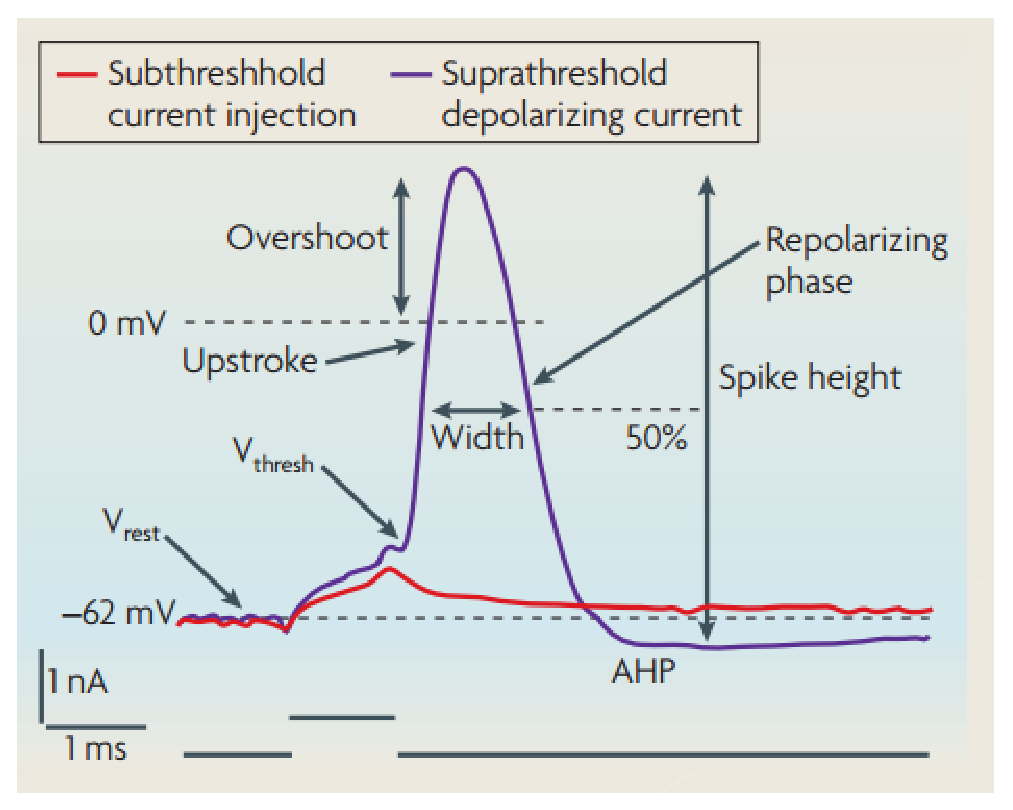
\includegraphics[height=6cm]{./images/AP_neuron.eps}}
 \caption{Anatomy of an AP in neuron}
\label{fig:AP_neuron}
\end{figure}

The shape of action potentials differs considerably among various types of
neurons in the mammalian brain, Fig.\ref{fig:AP_neuron}.
Dendrites probably also influence the form of somatically
recorded action potentials, partly by serving as a
capacitative load that slows and truncates fast spikes (by
absorbing currents that would otherwise go to changing
somatic voltage) but also by playing an active part in generating
afterdepolarizations.
 
 
Different neural behaviors are given in Fig.\ref{fig:neural_firing_behavior}
\begin{enumerate}
  \item tonic spike: Sect.\ref{sec:tonic-spike}) 
  
  \item tonic bursting: Sect.\ref{sec:tonic-bursting}) 
  
  \item phasic bursting: Sect.\ref{sec:phasic-spiking}
  
  \item mixed-mode firing: Sect.\ref{sec:mixed-mode}
  
  \item spike frequency adaptation: Sect.\ref{sec:spike-frequency-adaptation}
\end{enumerate}

\begin{figure}[htb]
  \centerline{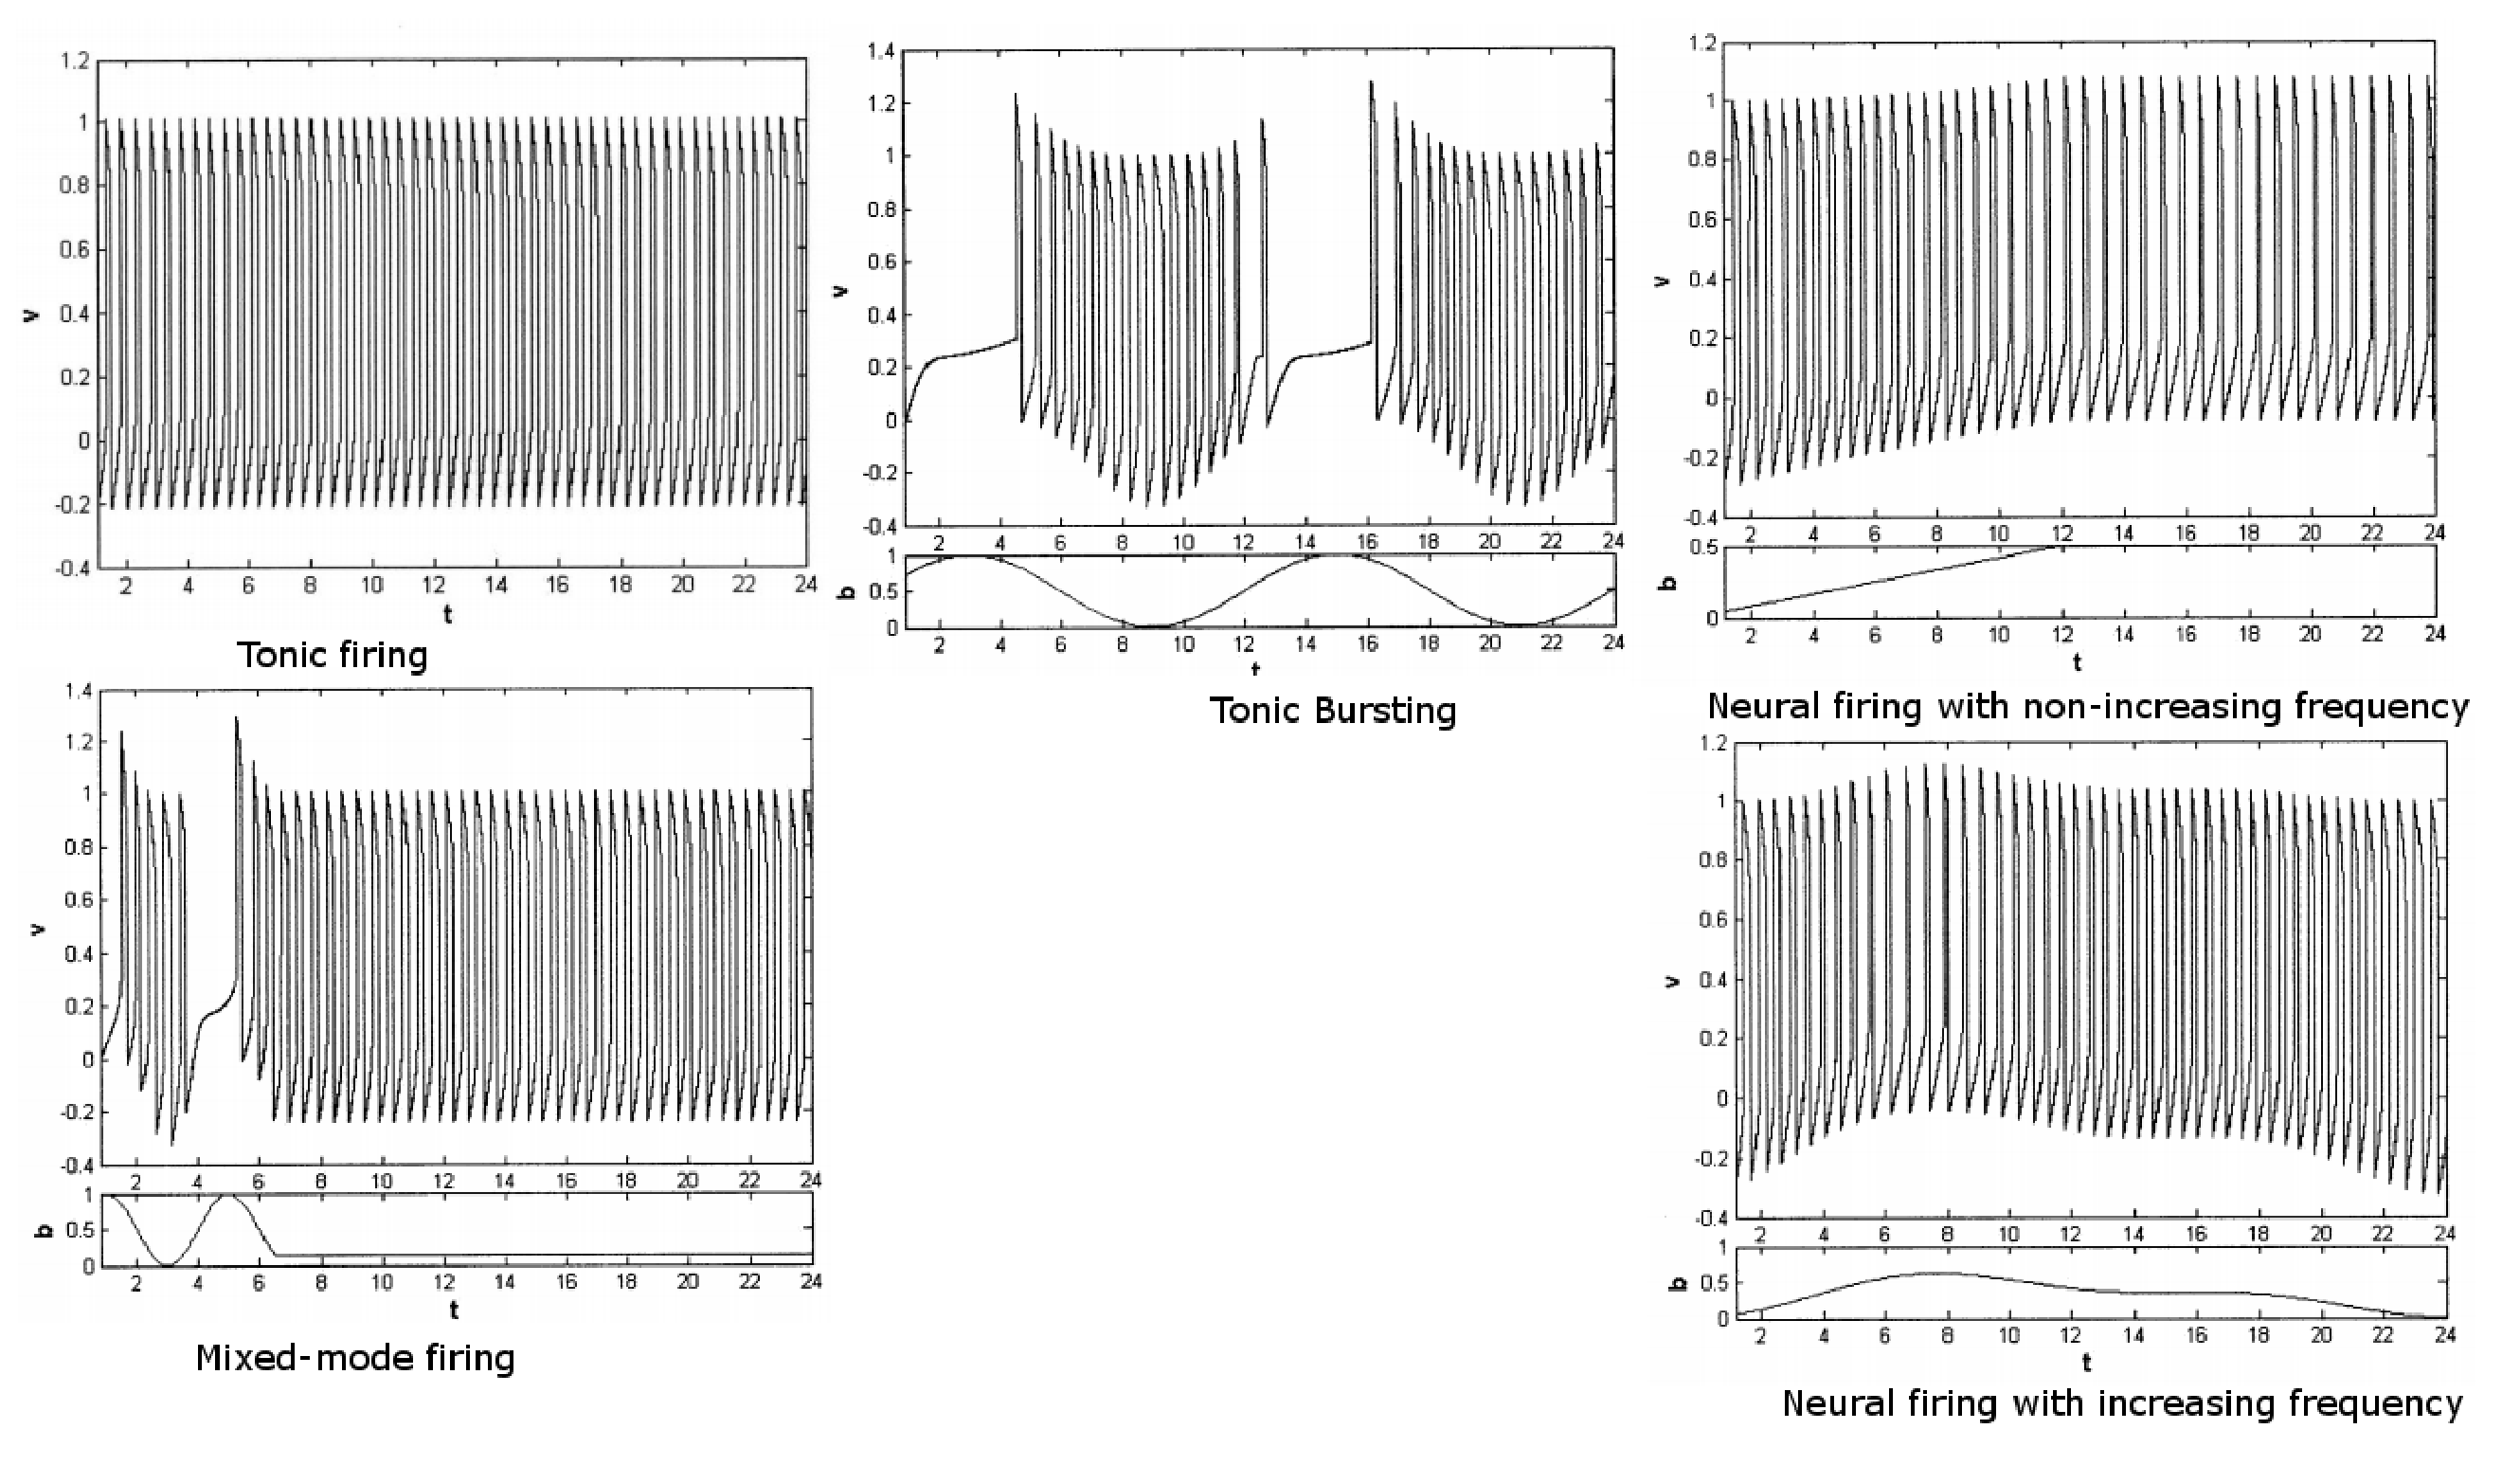
\includegraphics[height=6cm]{./images/neural_firing_behaviors.eps}}
  \centerline{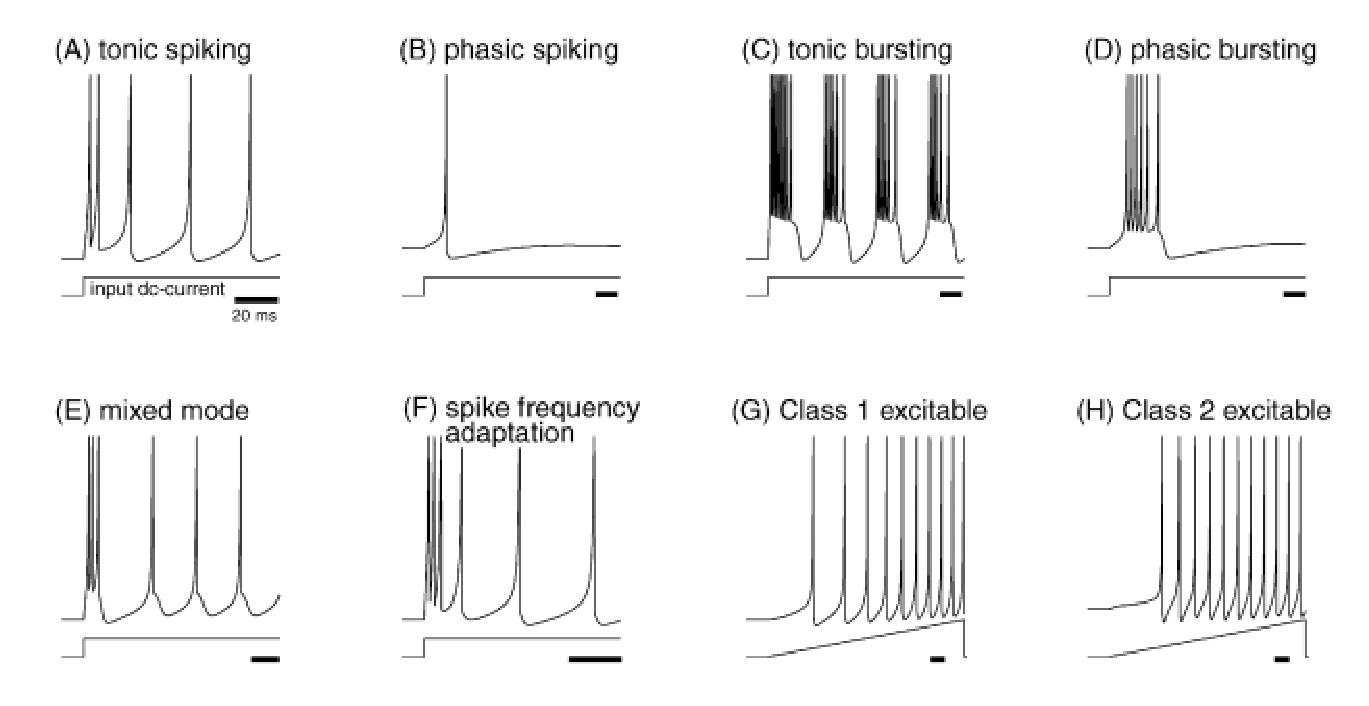
\includegraphics[height=4.5cm]{./images/neural_firing_behavior_1.eps}}
  \centerline{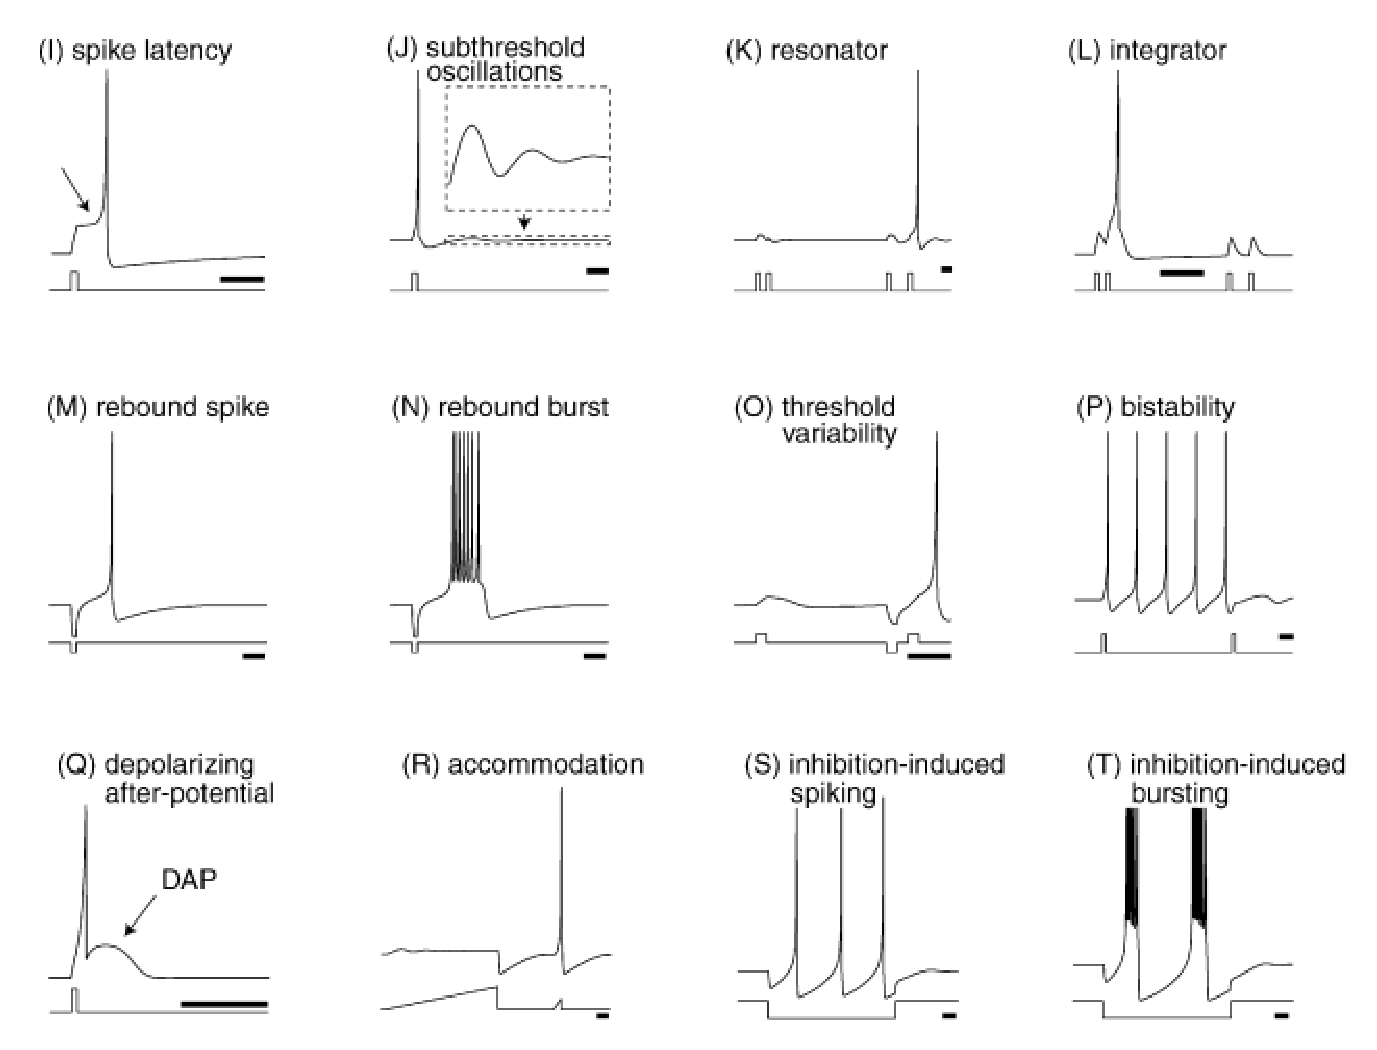
\includegraphics[height=7.0cm]{./images/neural_firing_behavior_2.eps}}
  \caption{Neural firing behaviors: (A) tonic firing (tonic spiking), (B) phasic
  firing (phasic spiking), (C) tonic bursting, (D) phasic bursting, (E) mixed
  mode, (F) spike frequency adaptation, (G) Class I excitable, (H) Class II
  excitable, (I) spike latency, (J) subthreshold oscillations, (K) resonator,
  (L) integrator, (M) rebound spike, (N) rebound burst, (O) threshold
  variability, (P) bistability, (Q) depolarizing after-potential (DAP), (R)
  accomodation, (S) inhibition-induced tonic spiking, (T) inhibition-induced
  tonic bursting}
  \label{fig:neural_firing_behavior}
\end{figure}

\clearpage


Spontaneous firing occurs in two distinct patterns, as shown in
Fig.~\ref{fig:firing_patterns}:
\begin{itemize}
\item solitary spikes (phasic spike), i.e. single spikes, interspersed with
periods of silences lasting as long as 30 sec
  
\item repetitive firing (bursts), which can be further divided into 
  \begin{enumerate}
  \item brief, i.e. tightly packed cluster of 2-4 spikes occuring at
    frequency up to 400/sec. 
    
  \item moderate duration, i.e. a train of 5-8 spikes with the
    underlying depolarization is 20-40 msec. and large 20-35mV. The
    first spike reach full size, but the latter ones are shorter and
    broader.
     
  \item prolonged bursts, i.e. a train of more than  10 spikes.
  \end{enumerate}
Notice that these subcategories overlap. 
\end{itemize}

\begin{figure}[hbt]
  \centerline{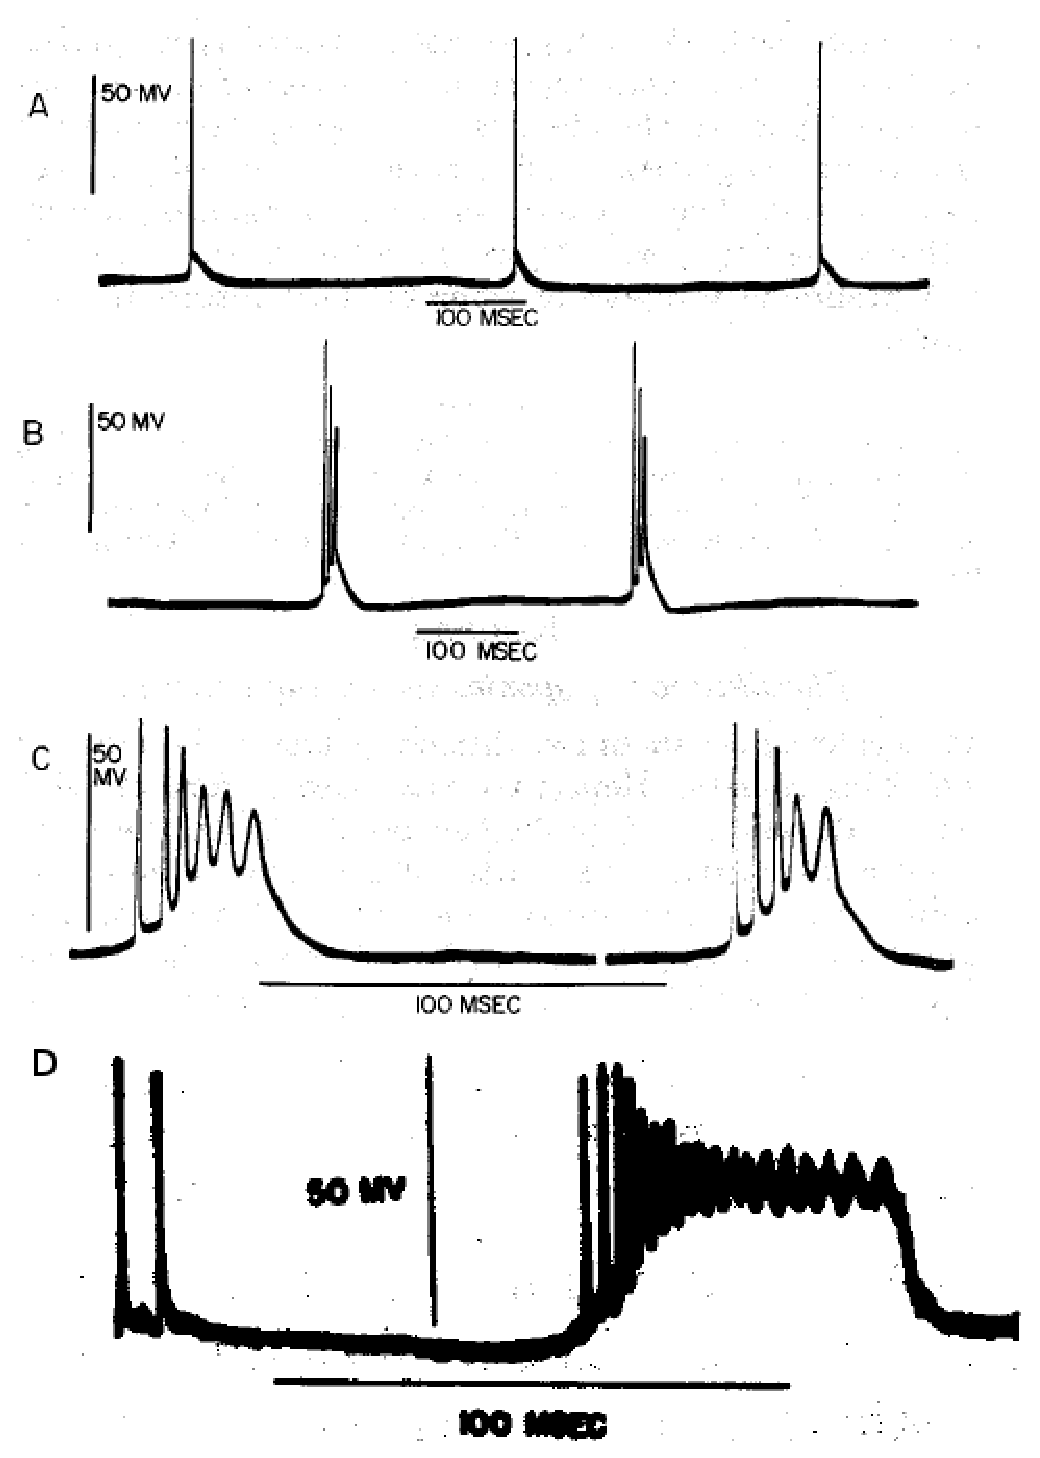
\includegraphics[height=5cm,
    angle=0]{./images/firing_patterns.eps}}
  \caption{(A) solitary spikes, (B) brief bursts, (C) moderate
    duration bursts, (D) prolonged burst}
\label{fig:firing_patterns}
\end{figure}

 
\begin{itemize}
  \item GABA ($\gamma$-aminobutyric acid)-releasing
interneurons in the cortex and hippocampus (Sect.\ref{sec:GABAergic-neurons}):
have a narrower spikes than glutamatergic neurons.

Cells with narrow spikes also commonly (but not always) display 'fast-spiking'
behaviour: being capable of firing at high frequencies with little decrease in
frequency during prolonged stimulation

Recently, the fast-spiking phenotype has been related to
expression of the Kv3 family of voltage-gated potassium
channels (Sect.\ref{sec:Kv_channel}). Kv3 channels help quickly repolarized the
membrane potential for the next spike.
 
   \item Glutamatergic neurons in the  subthalamic nucleus also have fast spike, 
    The neurons express large potassium currents mediated by Kv3-family
    channels.
    
    The calyx of Held, a presynaptic glutamatergic terminal, also has narrow
spikes with repolarization by Kv3 channels and can fire at high frequencies.

   \item 

\end{itemize}

Other than the shape of the spikes, the more important physiological property of
neurons is the firing pattern of a neuron (which includes frequency of
firing as a function of stimulus strength, bursting versus non-bursting activity
and adapting versus non-adapting behaviour) - Sect.\ref{sec:firing-pattern}.
However, the two cannot be cleanly separated, as differences in ionic
conductances producing differences in firing patterns will in general also
produce differences in spike shape, although these may be more subtle.

\textcolor{red}{Spike shape per se is probably most significant at presynaptic
terminals},  where small differences in shape can produce changes in the timing
of presynaptic calcium entry, leading to dramatic changes in postsynaptic
currents. Interestingly, presynaptic terminals can be quite different to that in
the cell body of the same neuron.

In the absence of stimulation, the cylindrical axon maintains a
constant potential difference, called {\bf resting potential} which
can be measured using two electrodes: one measures internal and one
measures external membrane potential, then amplified and recorded. The
resting potential is about -70mV in nerve cell
% $-65$mV in squid axons 
(in myocardial cells, it is $-90$mV).

At resting stage, all \ce{Na+}-channels, in axon hillock, are inactivated (the
availability is 100\%) while some \ce{K+}-channels are still open (leak channels
- allowing \ce{K+} to move outward {\it with rate as fast as their diffusion
through bulk water}), as shown in Fig.~\ref{fig:action_potential}. Between them,
\ce{Na+}-ion channels is low-voltage activated (LVA) channels\footnote{typically
15mV higher than the resting value,
  e.g. $E_m\approx -55$mV given that $E_r=-70$mV}
and response instantaneously. 


When 
\begin{itemize}
  \item an excitatory neurotransmitter (Sect.\ref{sec:neurotransmitter}) is
  released from the presynaptic neuron and binds to the postsynaptic denritic
  spines

When the positive charges travelling along the dendrites hits the axon hillock,
it depolarizes the membrane potential ($E_m$) here, i.e. making it
less negative.  As all ion-channels at the axon hillock are
voltage-dependent, such voltage changes can activate the ion channels,
leading to a positive feedback as when some of these channels open,
they allows the cations going inside the cell and triggers the
activations of other channels.
% {\it In nerve cells, the two major types of neuronal AP are \ce{Na+}
%   and \ce{K+} ion channels (cardiac action potential that will be
%   discussed \hyperref[sec:card-acti-potent]{later})}.
  
It means that when the membrane potential depolarizes, the first ion channels to
be activated are \ce{Na+}-ion channels.
As a result, some \ce{Na+} are first transported into the negatively charged
intracellular environment. This is a positive feedback process, i.e. the more
\ce{Na+} inside, the more positive the membrane potential, leading to more
\ce{Na+}-ion channels to open. The amount of influx \ce{Na+} will quickly
dominate the amount of efflux of \ce{K+} via the potassium leak channel.
  
  \item If a stimulus, in the form of a step current, is applied (in less than
millisecond duration) through a stimulating electrode touching the
membrane. 
\end{itemize}
The membrane potential will changes, i.e. $\Na$ channels open, which can make
the postsynaptic membrane potential depolarized. This depolarization travel
towards the soma and then axon hillock, diminishing exponentially with time -
time constant - and distance - space constant 
(similar to the concept of time constant) of less than a
centimeter~\cite{fitzhugh1969mmc} (Sect.\ref{sec:electrotonus_vs_transient}).

INFORMATION:
\begin{itemize}
\item With a weak stimulus: This is a {\it passive and local} response. 

% the membrane potential depolarized and then dies away with a time
% constant $\tau$ of about a millisecond. The potential decays away from the
% electrode with a ``space constant'' 

\item With a stronger stimulus, the membrane potential depolarize faster,
  yet still below +10mV - the threshold for AP. This is an {\it active and
  local} response.

\begin{figure}[hbt]
 \centerline{
\includegraphics[height=5cm]{./images/action_potential.eps}}
 \caption{The shape of action potential curve in squid axon}
\label{fig:action_potential}
\end{figure}
\end{itemize}

If several such stimulus events (i.e. signal reaches multiple postsynaptic of
the nerve cell) occur in a short time or with a much stronger stimulus, the
membrane potential can depolarize above a threshold, the potential abruptly
increase $\Delta V$=100mV and form a triangular waveform, lasting about a
millisecond, as shown in Fig.~\ref{fig:action_potential}. Such a curve is called
{\bf action potential} (AP).

The \ce{K+}-channels (Chap.\ref{chap:K_model}) is of type HVA channels and its
state changes slowly. These channels do not close right away when the membrane
returns to its normal resting potential (typically -70mV); some \ce{K+}
continues to flow out causing a more negative value than the resting potential.
This is the unusual state - referred to as {\it refractory state} to that many
literatures don't mention. During this time, a second stimulus, no matter how
strong, cannot produce a second impulse, i.e. many ion channels are unable to
open again.
During this time, no AP can begin - {\it undershoot phase} (or absolute
refractory period).  This undershoot phase ensure the AP only propagate down the
axon, not to back it up.  Following the absolute refractory period is the {\it
relative refractory period}, during which a second stimulus can produce an
impulse, yet the stimulus must be more stronger as the threshold is higher than
that of the resting membrane. During this relative refractory period, the
threshold gradually falls until it returns to the same threshold of the original
resting phase.  Indeed, the AP spikes an electrical current which propagates
along the axon that we will studied shortly.


This transient (impulse) splits into two separate waves travelling away
from the
stimulating electrode in two opposite directions along the fiber at a constant
conductance velocity\footnote{the structure of nerve cells and other excitable
cells guarantee the signal to be transmitted in 2D, not in 3D}.
When an impulse travels, it can be recorded at any point along the fiber as it
passes. However, it is impossible to deduced where it originated or the strength
of the stimulus that produced it. Hence, the fact that one can confirm only the
presence or absence of the impulse, is called the {\it all-or-none law}.

% In nerve cells, a typical AP is initiated at the axon hillock when the
% membrane is depolarized enough (i.e. $E_m$ increase
% sufficiently). This process is described as follows.  

%Now, we will discuss in detail the mechanism in neuron. 




% \begin{figure}[htb]
%   \centerline{\includegraphics[height=12cm]{./images/Action_potential_vert.eps}}
%   \caption{Action potential. (A) schematic diagram (yellow: weak
%     stimulus, orange: strong stimulus that trigger AP. (B) real
%     AP}\label{fig:action_potential_2}
% \end{figure}


{\bf Properties}:
\begin{enumerate}
\item ``all-or-none'' principle: the amplitude of an AP is independent
  from the current which produced it. Therefore, an AP is said to be
  {\it all-or-none}, since they either occur fully or they do not
  occur at all. Instead, the frequency of AP is what encodes for the
  intensity of a stimulus.

\item pacemaker potential: some excitable cells do not require stimuli
  to fire AP: they spontaneously depolarize their axon hillock and
  fire AP at a regular rate, like an internal clock. Although such
  pacemaker potential have a natural rhythm, they can be modified by
  external stimuli.

\item phases: the course of an AP can be divided into 5 parts: {\it
    rising phase}, {\it peak phase}, {\it falling phase}, {\it
    undershoot phase}, and finally the {\it refractory period}.

\item voltages and currents of AP in all of its phases were modeled by
  Hodgkin and Huxley (1952). However, they considered only 2 types of
  voltage-gated ion channels and make several assumptions about them
  that many of them are not true in nature.

\item there are many types of voltage-activated \ce{K+} channels in
  neurons, some of them inactivate fast (A-type) and some of them
  inactivate slowly or not inactivate at all.
\end{enumerate}


{\bf Myelin sheaths}: Myelin sheaths were there, along the axon, to
ensure there is no leakage of the electric current through the ion or
leak channels. Nevertheless, to ensure the signal does not fail, the
signal is also boosted by the means of {\it nodes of Ranvier} between
myelin sheaths.  The mechanism of the nodes of Ranvier is as
follows. As the AP reach the nodes of Ranvier, it depolarizes the
membrane. With the same process as that at the axon hillock, a new AP
is triggered. When the AP reach the ends of the axon, it trigger the
release of neurotransmitters into the synaptic cleft. This may
combine with other inputs to provoke a new action potential in the
post-synaptic neuron or muscle cells.


Lastly, calcium cations and chloride anions are invoked in other types
of action potentials, i.e. \ce{Ca^2+} in cardiac AP, \ce{Cl-} in AP of
some algae\cite{mummert1991api}.
% In general, the flowing of charges (neurotransmitters) that activates
% the voltage-gated ion channels is called action potential (AP). To
% visualize the whole process, Fig.\ref{fig:action_potential} shows an
% acute upward slope in the rising phase and a slowly downward slope in
% the falling phase, then a gradually rising in the membrane potential
% at the undershoot phase.


% \begin{figure}[htb]
%   \centerline{
\includegraphics[height=6cm]{./images/action_potential.eps}}
% \caption{Action potential (review)}\label{fig:action_potential_1}
% \end{figure}

% , as having (protein) ion channels in its membrane. And it
% is these channels which give rise to the resting potential that we
% discussed in the preceding
% % The reason that the
% % combination of both chemical and electrical change leads to the name
% % electrochemical
% % signal\footnote{http://faculty.ucc.edu/biology-potter/Neuron/sld001.htm}. In
% % the end of the process, the neurotransmitter will be re-uptake back to
% % the axon terminal.
 
% \begin{figure}[htb]
% \centerline{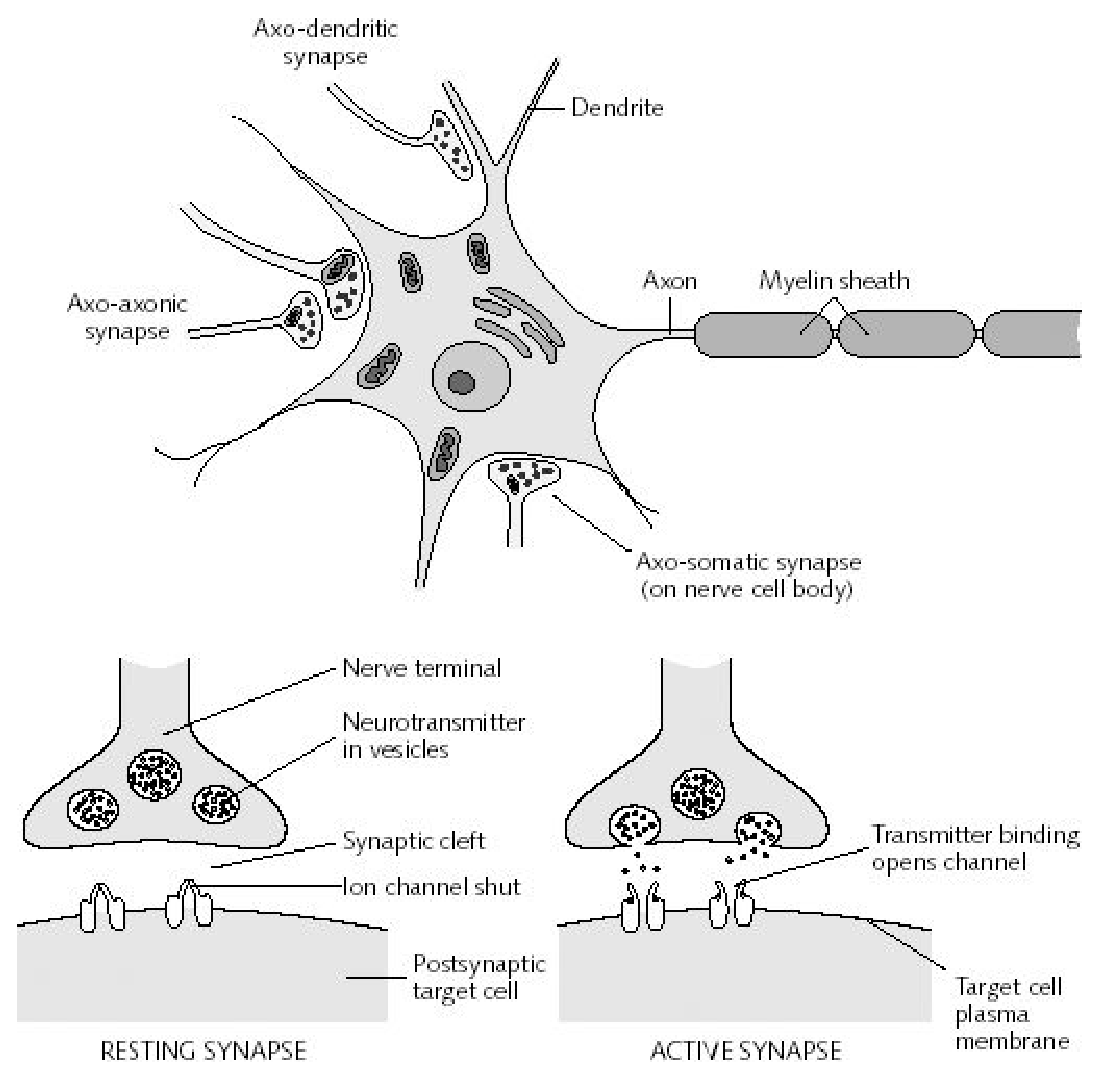
\includegraphics[height=7cm]{./images/synapse2.eps}}
% \caption{Transmission process in synapses}\label{fig:synapse2}
% \end{figure} 

In nerve cells, we can observe different characteristic
of AP
\begin{itemize}
\item phasic spiking = a single AP
\item tonic spiking = a train of spikes
\item burst = a train of spikes
\item 
\end{itemize}

\subsection{** tonic spiking}
\label{sec:tonic-spike}

The nerve cell is injected pulses of DC current via electrode attached to the
neuron, once the input is on, the neuron continues to fire a train of spikes, 
at a given frequency.
This kind of behavior, called {\bf tonic spiking}, can be observed in the three
types of cortical neurons
\begin{enumerate}
  \item regular spking (RS): excitatory neuron
  
  \item low-threshold spiking (LTS): 
  
  \item fast spiking (FS): inhibitory neurons
\end{enumerate}
So, continuous firing of such neurons indicate that there is a persistent input

We also have inhibition-induced tonic spiking,
Fig.\ref{fig:neural_firing_behavior} (S).

The frequency of tonic spiking can be constant (this section) or adapted.
Sect.\ref{sec:tonic-spike-frequency-adapted} discusses adapted frequency.
When the frequency depends on the strength of the input, still the input is
above the threshold, we have Class I excitability
(Sect.\ref{sec:Class-I-excitability}).

\subsection{** tonic bursting}
\label{sec:tonic-bursting}

Some neurons, such as the chattering neurons in cat neocortex
[7], fire periodic bursts of spikes when stimulated.
Here, neurons fires a certain number of spikes and is silent for a certain
amount of times; and then it repeats this pattern in a periodic manner.
The interburst (i.e., between bursts) frequency may be as high
as 50 Hz, and it is believed that such neurons contribute to the
gamma-frequency oscillations in the brain

We also have inhibition-induced tonic bursting,
Fig.\ref{fig:neural_firing_behavior} (T)
(Sect.\ref{sec:inhibition-induced-firing}).

\subsection{** phasic spiking (single spike)}
\label{sec:phasic-spiking}

A neuron may fire only a single spike at the onset of the input, and remain
quiescent afterwards. It is useful for detection of the beginning of
stimulation.

In some neuron, this phasic spiking can be the result of a brief inhibitory
input (Sect.\ref{sec:rebound-spike}).

In some neurons, there can be a delay before the spike to occur
(Sect.\ref{sec:spike-latency}), and after depolarizing phase, it can be AHP or
DAP (Sect.\ref{sec:depolarizing-after-potential}).
\subsection{** phasic bursting (single burst)}
\label{sec:phasic-bursting}

Similarly  to  the  phasic  spikers,  some  neurons  are  phasic
bursters, i.e. a single burst. Such neurons report the beginning of
the stimulation by transmitting a burst.

In some neuron, this phasic bursting can be the result of a brief inhibitory
input (Sect.\ref{sec:rebound-burst}).


\subsection{** mixed mode: bursting + spiking}
\label{sec:mixed-mode}

Intrinsically bursting (IB) excitatory neurons in mammalian
neocortex can exhibit this mixed mode behavior.

The neuron fires a single  burst (Sect.\ref{sec:phasic-bursting}) at the
onset of the stimulation, and then switch to tonic spiking
\citep{izhikevich2004}.

\subsection{** spike frequency adaptation (broadening of AP during repetitive
firing)}
\label{sec:tonic-spike-frequency-adapted}


Broadening of neuronal action potentials during repetitive firing is a
widespread phenomenon in somata, dendrites and nerve terminals (Aldrich et al.
1979; Gainer et al. 1986; Jackson et al. 1991; Andreasen \& Lambert, 1995; Ma \&
Koester, 1996).

\begin{itemize}

  \item  Hippocampal pyramidal cells in behaving rats fire brief bursts of 2-10
  action potentials at frequencies of 100-300 Hz, during which the spikes
  typically become broader towards the end of the burst (Fox \& Ranck, 1981)
  
\end{itemize}

Since most of the influx of $\Ca$ typically occurs during the late part of each
action potential (Llinas et al. 1982), spike broadening is an efficient way of
increasing $\Ca$ influx, thus modulating intracellular $\Ca$ signals and
$\Ca$-dependent ion channels, enzymes, second messengers cascades, gene
transcription, and release of transmitters and hormones.

This is a variant of tonic spiking (Sect.\ref{sec:tonic-spike}) where 
the nerve cell first fire relatively high at the onset of stimulation, and then
it adapts.

This is found in regular spiking (RS) neuron
(Sect.\ref{sec:regular-spiking-pattern}). Low-threshold spiking (LTS) inhibitory
neurons also have this property. The interspike frequency of such cells may
encode the time elapsed since the onset of the input.

Spike broadening during repetitive firing in neurones is often due to 
\begin{itemize}
  \item  cumulative
inactivation of voltagegated $\K$ channels, including slowly inactivating
'delayed rectifier' $\K$ channels - Sect.\ref{sec:delay-rectifier}) (Aldrich et
al. 1979)

This mechanism has been described in a variety of neurones, including molluscan
somata (Aldrich et al. 1979; Ma \& Koester, 1996), magnocellular hypothalamic
neurones (Bourque \& Renaud, 1985) and pituitary neurosecretory terminals
(Jackson et al. 1991)

  \item fast-inactivating $\K$ channels (A-channels -
  Sect.\ref{sec:A-type-K+current}) (Jackson et al. 1991; Ma \& Koester, 1996).

This mechanism has been described in a variety of neurones, including molluscan
somata (Aldrich et al. 1979; Ma \& Koester, 1996), magnocellular hypothalamic
neurones (Bourque \& Renaud, 1985) and pituitary neurosecretory terminals
(Jackson et al. 1991); and recently in CA1 pyramidal neurons.
  
  \item enhanced activation of voltage-gated $\Ca$ channels late in the train

  \item rapidly inactivating BK current:
  
The hypothesis that  BK-type K+ channels, which are involved in spike
repolarization, also contribute to the spike broadening during repetitive firing
was test by Shao et al. (1999).

\end{itemize}

\subsection{** Class I excitability}
\label{sec:Class-I-excitability}


Class I excitability is a variant of tonic spiking (Sect.\ref{sec:tonic-spike})
in which the frequency of tonic spiking of neocortical RS excitatory
neurons depends on the strength of the input, and it may span 
the range from 2 Hz to 200 Hz, or even greater.

Class 1 excitable neurons can encode the strength of the input into
their firing rate. NOTE: The input strength still must be greater than the
firing threshold. 
So, here, their firing rate is a good predictor of the strength of
stimulation.

\subsection{** Class II excitability}
\label{sec:Class-II-excitability}


Unlike Class I excitability (Sect.\ref{sec:Class-I-excitability}), 
Class II excitability neurons behave in a way that either no firing
(quiescent) or firing with a a train of spikes with a certain
relatively large frequency, say 40 Hz, at weak input.
So, here, their firing rate is a poor predictor of the strength of
stimulation.

 
\subsection{** Spike latency (large ramp before spike)}
\label{sec:spike-latency}

Most cortical neurons display a large ramp before the spike, i.e. 
fire spikes with a delay that depends on the strength of the input signal.
Here, following a brief depolarizing pulse, the neuron fires not during the
pulse but after it.

The RS cells in mammalian cortex can have latencies of tens of ms. Such
latencies provide a spike- timing mechanism to encode the strength of the input


\subsection{** Subthreshold oscillation (membrane potential oscillation)}
\label{sec:subthreshold-scillation}

Practically every brain structure has neurons capable of having oscillatory
potentials. The frequency of such oscillations play an important role and such
neurons act as bandpass filters.

Neurons having this subthreshold oscillation can serve as a resonator, i.e. only
trigger the AP once the input is of the same frequency of the subthreshold
oscillation (Sect.\ref{sec:frequency-preference}).

The neurons that does not have this subthreshold oscillation typically serve as
an integrator (Sect.\ref{sec:coincidence-detectors})


\subsection{** Frequency preference (resonance)}
\label{sec:frequency-preference}

Some neurons having oscillatory potentials
(Sect.\ref{sec:subthreshold-scillation}) can respond selectively to the inputs
having frequency content similar to the frequency of subthreshold oscillations,
Fig.\ref{fig:neural_firing_behavior}(K).

Such neurons can implement frequency-modulated (FM)
interactions and multiplexing of signals. Such  neurons  are  called
resonators.

\subsection{** Coincidence detector (integrator)}
\label{sec:coincidence-detectors}


The neuron that doe not have oscillatory potentials
(Sect.\ref{sec:subthreshold-scillation}) prefer  high-frequency  input;  the 
higher  the  frequency the more likely they fire. This can be useful for
detecting coincident or nearly coincident spikes.

\subsection{** Rebound spike (after brief inhibition)}
\label{sec:rebound-spike}

After being received and released from an inhibitory input, 
in response to this brief inhibitory input, some neurons may fire a spike
(rebound spike or post-inhibitory spike)

This phenomenon is related to the anodal break excitation in excitable
membranes. Many spiking neurons can fire in response to brief inhibitory inputs
thereby blurring the difference between excitation and inhibition.

\subsection{** Rebound burst (after brief inhibition)}
\label{sec:rebound-burst}

Some neurons, including the thalamo-cortical cells, may fire post-inhibitory
burst. It is believed that such
bursts contribute to the sleep oscillations in the thalamo-cortical
system.

\subsection{** Threshold variability (in firing)}
\label{sec:threshold-variability}

It is well-known that biological neurons have a  variable  threshold  that 
depends  on  the  prior  activity  of  the neurons.

Suppose a given stimulus input (e.g. 10mV depolarization for 1ms) per se does
not lead to a firing. But if we precede this input with a brief inhibitory
input, neuron fires  the second time because  its ``threshold'' was lowered by
the preceding inhibitory input.

Hence, the same 10-mV depolarization for 1ms can be subthreshold or
superthreshold depending on the prior activity. Interestingly, a preceding
excitatory pulse might raise the threshold and make the neuron less excitable.

\subsection{** Bistability (resting + spiking states)}
\label{sec:bistability-rest-vs-spiking}

The neuron can switch between tonic spiking state and quiescent state by the
brief excitatory input, Fig.\ref{fig:neural_firing_behavior}(P).

\subsection{** Prolonged Depolarizing after-potential (DAP) or 
after-hyperpolarization (AHP))}
\label{sec:depolarizing-after-potential}
\label{sec:after-hyperpolarization}

After firing a spike, the membrane potential of a neuron may exhibit a prolonged
after-hyperpolarization (AHP or a.h.p.) or a  prolonged  depolarized 
after-potential (DAP).

AHP is due to an increased \ce{K+} conductances, possibly activated by the
inward flux of \ce{Ca^2+} leading to the opening of $\Ca$-dependent $\K$
current ~\cite{connor1982epn}.

Previous studies have demonstrated three types of AHP in hippocampal pyramidal
cells
\begin{enumerate}
  \item $\Ca$-dependent slow AHP (Hotson \& Prince, 1980; Alger \& Nicoll, 1980),
  
  \item shorter, $\Ca$-independent AHP (Gustafsson \& Wigstrom, 1981).
  
  \item fast $\Ca$-dependent AHP (Storm, 1987) a direct continuation of the
  spike repolarization ('spike undershoot'), has been observed during repetitive
  firing in CAl cells. 
  
  This is also found in neocortex (Schwindt, Spain, Stafstrom, Chubb \& Crill,
  1984).
\end{enumerate}



A tonic spike has DAP (read more at Sect.~\ref{sec:hap-ahp-dap}) of
approximately 10mV in amplitude and 30msec. in duration. The presence
of DAP is very consistent although its parameters vary from cell to
cell. In fact, DAP summate when multiple firing occurs. 


The semilogarithmic plot of decay of DAP following one and burst of 3
and 6 spikes is shown in Fig.~\ref{fig:semilog_plot} . The lines are
parallel indicates that the time constant of decay is insensitive to
the number of spikes, and the mean time constant was 14.5 msec
(measured in 10 cells).

\begin{figure}[hbt]
  \centerline{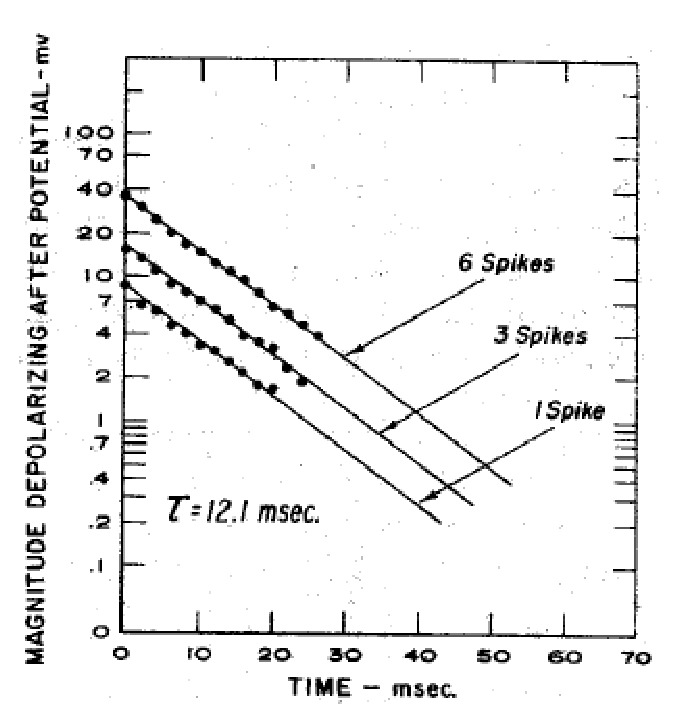
\includegraphics[height=5cm,
    angle=0]{./images/semilog_plot.eps}}
\caption{Semilogarithmic plot of decay of DAP}
\label{fig:semilog_plot}
\end{figure}

\subsection{** Accomodation (sensitive to brief coincident inputs, but not to
slowly increasing input)}
\label{sec:coincidenct}

The slowly ramped current in the figure Fig.\ref{fig:neural_firing_behavior}(R)
does not elicit a spike, while a smaller but sharply ramped current elicits a
spike.

During the slow ramp, the inward currents have enough time to inactivate and
outward currents have enough time to activate, so the neuron accommodates,
becomes less excitable and cannot generate a spike

\subsection{** Inhibition-induced firing (spike or burst)}
\label{sec:inhibition-induced-firing}
\label{sec:inhibition-induced-spike}
\label{sec:inhibition-induced-burst}

A bizarre feature of  many thalamo-cortical neurons  is that they are quiescent
when there is no input, but fire when hyperpolarized by an inhibitory input or
an injected current.

\begin{itemize}
  \item tonic spiking: the injected current activates the h-current and deinactivates calcium T-current,
leading to tonic spiking
 
  \item tonic bursting: instead of spiking, a thalamo-cortical neuron can
fire tonic bursts of spikes in response to a prolonged hyperpolarization

\end{itemize}
It is believed that such bursting takes place during
spindle wave oscillations in the thalamo-cortical system and it
plays an important role in sleep rhythms.

\subsection{back-propagating action potential (bAP)}
\label{sec:bAP}
\label{sec:back-propagating_AP}


Once the AP is initiated in the axon initial segments (Sect.\ref{sec:AIS}), the
action potential can also propagate back to the soma and then into the dendritic
tree in a retrograde fashion.
This is called {\bf back-propagating action potential} (bAP)
\citep{spruston1995}.
Back-propagating action potentials might signal the occurrence of recent
neuronal excitation and influence synaptic plasticity.

Kv channels (Sect.\ref{sec:Kv_channel}) and hyperpolarization-activated cyclic
nucleotide-gated (HCN) cation channels (Sect.\ref{sec:HCN-channels}) on
dendrites further control action potential back-propagation, and the time course
and extent of the passive spread of synaptic potentials, leading to long-term
potentiation
 (LTP) or long-term depression
 (LTD) depending on the timing of the back-propagating action potential relative to the
synaptic input (Sect.\ref{sec:STDP}).


bAP has found its role in synaptic plasticity by changing
the probability of synaptic activation under the same presynaptic stimulus
(Sect.\ref{sec:synaptic_plasticity}) under the mechanism spike-time dependent
plasticity (STDP - Sect.\ref{sec:STDP}).

The extent of this action potential backpropagation has been found to vary
depending on the type of neuron, depending on
\begin{itemize}
  \item density of $\Na$ channels in the dendrite
  
  \item dendritic morphology and branching pattern
  
  \item somatic AP shape: the broader an event the less it will attenuate as it
propagates into the dendritic tree.
\end{itemize}
The study showed that backpropagation into the dendritic tree is most effective
in the {\bf dopamine neurons of the substantia nigra}
(Sect.\ref{sec:dopaminegic_neurons}), which have the broadest somatic action
potentials of all neurons in which action potential backpropagation has
been studied \citep{stuart1997}.

Some neurons have backpropagating action potentials, while others do not. This
cell-specific difference suggests that active backpropagation of action
potentials into the dendritic tree is functionally important in those neurons
where it occurs. \textcolor{red}{What bAP does?}
\begin{itemize}
  \item provide a retrograde signal to the dendrite tree indicating the level of
  neuronal output (e.g. in long-term potentiation
  Sect.\ref{sec:glutamate_receptor}).
  
  \item cause an increase in $\Ca$ in the dendritic spines which beside induct
  certain form of synaptic plasticity, influence synaptic integration by
  downregulating NMDA receptor-mediated responses or by activating dendritic
  efflux $\K$ conductances which could shunt out parts of the dendritic tree
  (explained by the increase of extracellular $[\K]$ due to $\K$ channel opening
  that depolarize presynaptic terminals, thereby transiently influencing
the probability of transmitter release).

   \item \ldots 
\end{itemize}



\subsection{Mechanism of signal transmission}
\label{sec:neuron_mechanism_transmission}

Nerve axons can tranmist AP over a long distance without attenuation,
Fig.\ref{fig:nerve_cell}.
The amplitude of AP in nerve axon is about +100 mV with duration 1ms (from -75
mV to +55 mV).


\begin{figure}[hbt]
  \centerline{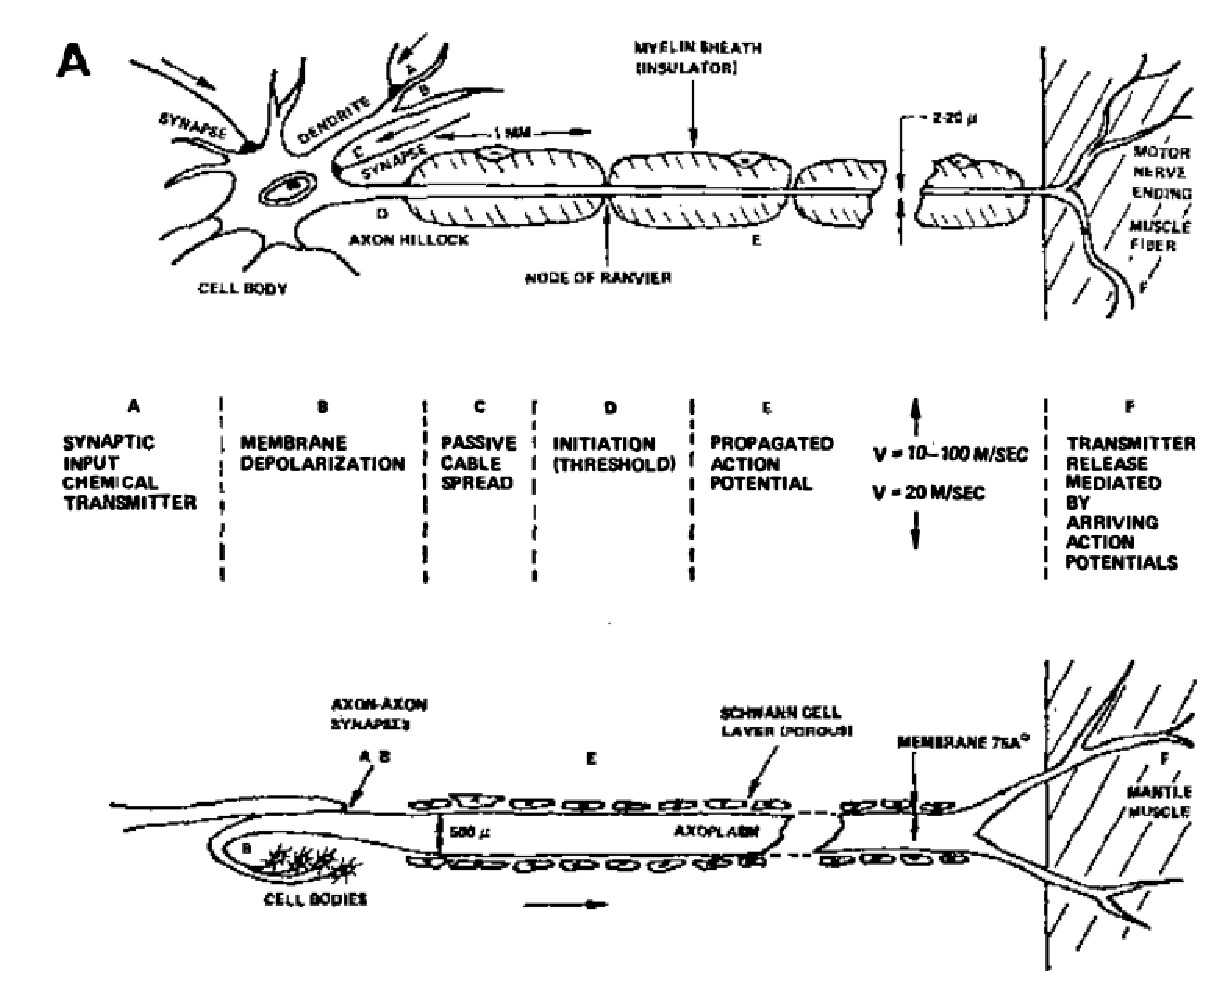
\includegraphics[height=7cm]{./images/nerve_cell.eps}}
  \caption{Transmission of information in a vertebrate myelinated nerve and in
  cephalapod giant nerve \citep{ehrenstein1972}}
  \label{fig:nerve_cell}
\end{figure}

In an excitable cell, electrical signals are carried primarily by
transmembrane ionic currents, which result in changes in transmembrane
voltage. These ionic currents involve mainly \ce{Na+}, \ce{K+},
\ce{Ca^2+}, \ce{Cl-} whose movements are governed by physical laws.

At rest, $\Na$ channels close and $\K$ channels still active. The resting
potential is about -75 mV, while the reversible potential of $\K$ channels
is slightly more positive than that. During an AP, the membrane conductance
increases by a factor of 40. The value +55 mV is the reversible potential for
$\Na$ channels. 

If the membrane is ideally permeate to a single ion, the formula for membrane
potential at equilibrium is Nernst equation (Sect.\ref{sec:nernst-equation}). In
vivo, the membrane permeate selective and to more than one type of ions. So, the
widely used formula for membrane potential at equilibrium is constant-field
theory where the logarithm is replaced by a weighted sum of ionic activities
(Sect.\ref{sec:GHK_current}).

Due to the selectivity of the membrane, the nerve membrane serve as a battery.
This battery is continuously recharged by metabolic active-transport
``pumps". The main function of the pump is to restore the steady-state after the
ionic exchanges during AP. A 0.1$\mum$ axon termincal will double $[\Na]_i$
after 10 impulses, while a giant axon can support up to $3\times 10^5$ impulses
\citep{ehrenstein1972}.

Membrane permeability are specified via conductances which are
expressed in terms of the current-voltage relation (I-V). There are
two behaviors: linear and nonlinear. In most cases, we assume the
relation I-V is linear (i.e. ohmic), the relation is
\begin{eqnarray*}
  I = gV
\end{eqnarray*}
In subthreshold condition, $g$ is a constant. In transthreshold
condition, i.e. when the change in membrane voltage is positive
enough, it may lead to the generation of {\bf action potential}, the
primary form of electrical signals in excitable cells; $g$ is a
function of time and $V_m$. At first, we examine different basic
physical laws.

% \section{Membrane time constant}
% \label{sec:membr-time-const}

% As the voltage at the soma (body) can be measured experimentally with
% greater ease than those in dendrite network, and further, it is the
% voltage at the soma that determine whether or not the neuron fires an
% action potential. The electrodes are injected into the soma and
% they measured the steady current flows across the soma membrane. The
% result showed it was only a small portion; a major portion flow into
% the several dendritic trees and then out across the extensive
% dendritic membrane surfaces.

% Under the subthreshold condition, the soma membrane is modeled as a
% lumped-RC. The membrane time constant $\tau$ is defined as the product
% of the passive membrane resistance $R_m$ and capacitance $C_m$.
% \begin{eqnarray}
%   \label{eq:517}
%   \tau = R_mC_m
% \end{eqnarray}

\subsection{Bistability}
\label{sec:bistability}

The essential ingredients for bistability are positive feedback and cooperativity
\begin{enumerate}
  \item Positive feedback greatly amplifies a stimulus once it is above threshold. 
  
  \item Cooperativity is required to generate the threshold. The higher the
  cooperativity, the better is the rejection of spurious triggering events
  
\end{enumerate}
\textcolor{red}{However, those are not enough to trigger calcium spiking}
(Sect.\ref{sec:calcium-oscill-waves}).


Example of Action Potential (Sect.\ref{sec:action-potential})
\begin{enumerate}
  \item  In action potentials, positive feedback results from depolarization and
Na+ channel opening, which are mutually reinforcing ({\bf positive feedback
loop}).

  \item Cooperativity comes from the steep voltage dependence of channel
  opening, which results from the concerted movement of the four voltage sensors
  in the channel
  
The falling phase of action potentials is a consequence of the inactivation
of Na+ channels and the opening of K+ channels.
These deactivation processes terminate the positive-feedback loop that produces
the rising phase.

  \item Deactivation results in a refractory period, in which the system
cannot be triggered or can be triggered only at a much higher threshold

The responsiveness of the system is restored by reactivation processes,
namely reactivation of Na + channels and closure of K + channels after
repolarization. 

The period between spikes in a train of action potentials is
determined by the time course of deactivation and reactivation, and by
the stimulus intensity.
\end{enumerate}

Example of cAMP secretion triggering many thousands of slime mold cells
together to form a slug in times of starvation
\begin{enumerate}
  \item The stimulation of cAMP secretion by the binding of cAMP to cell-surface
  receptors of Dictyostelium discoideum generates a positive-feedback loop
  
  \item Deactivation here results from phosphorylation of the occupied receptor,
  probably by PKC
  
  
  \item The system is reactivated by dephosphorylation of the receptor.
  
This sequence of positive
feedback followed by deactivation and reactivation leads to minute-long
pulses of cAMP in the extracellular milieu every six minutes.

  \item Waves of cAMP lead to waves of cells moving towards the aggregation
  center, the site at which cAMP was first secreted
\end{enumerate}

Example of $\Ca$ spike: two plausible models
\begin{enumerate}
  \item  IP3-Ca2+ crosscoupling model (ICC model)

\begin{enumerate}
  \item a positive feedback comes from the mutual reinforcement
of IP3-induced Ca2+ release and Ca2+ -stimulated IP3 formation

  \item 
\end{enumerate}
  
  \item calcium-induced calcium release model (CICR model) - calcium influx is
  important 
  
\end{enumerate}


\section{Ionic conductances}
\label{sec:volt-activ-ionic}

The elementary bioelectrivity of mammalian neurons are determined by
some voltage-activated and ligand-activated ionic conductances.  The
very first studies looked at dendritic excitability,
i.e. \ce{Ca^2+}-dependent spikes in avian Purkinje cell dendrites and
mammalian neurons~\cite{llinas1988iep}.

The low-threshold \ce{Ca^2+} conductance is essentially inactivated at
resting potential, and deinactivated by membrane hyperpolarization. In
deed, a subthreshold depolarization can also produce an action
potential (AP) if superimposed on either a depolarizing or
hyperpolarizing membrane potential change. 

The non-inactivating or persistent \ce{Na+} conductance can generate
long, low-amplitude {\it plateau potentials}, which can regulate
excitability.

In addition to the inward \ce{Na+} and \ce{Ca^2+} ions, there is also
outward currents generated by \ce{K+} conductances. However, in
contrast to \ce{Na+}, the kinetics, voltage-dependence, single-channel
behavior of \ce{K+} vary widely. The reason is that there are many
type of \ce{K+} channels found in the same
cells\footnote{read Appendix of Thermo-Stat book}. Although, K, Ca and
  even Na channels are found in also non-excitable cells, K channels
  seem to be the most ubiquitous~\cite{rudy1988duk}.

  In nerve cells, there are many different firing patterns of AP under
  different length of squared current impulses. Such patterns are
  examined at single-cell level and a network of interconnected nerve
  cells.  Repetitive firing has been consistently observed in CNS
  under normal
  condition~\cite{kandel1961ehn_b, connor1971prf, connor1982epn}.

\section{Information encoding in firing patterns}
\label{sec:firing-pattern}

Unpon a given input, the nerve cells, at different regions the brain, can
trigger the AP with different firing patterns: bursting versus non-bursting
activity and adapting versus non-adapting behaviour
(Sect.\ref{sec:AP-neuron-soma}).
\begin{itemize}
  \item  Most neuronal cell bodies (in both vertebrate
and invertebrate animals) can fire over a far wider range
of frequencies and can respond to small changes in input
currents with significant changes in firing frequency.
  
  \item The membrane of squid axon is a poor encoder, as it fires
only over a narrow range of frequencies when stimulated
by the injection of widely-varying current levels.

However, some other invertebrate axons
can fire over a wide frequency range and have a richer
repertoire of ion channel type.
\end{itemize}
As a result, APs serve a very different function in neuronal
cell bodies, where they encode information in their
frequency and pattern, than in axons, where they serve
primarily to rapidly propagate signals over distance



% Under long intracellular pulses at different stimulated current
% intensities, we observe different firing patterns
There are two interested questions~\cite{kandel1961ehn_c}:
\begin{enumerate}
\item the level of membrane depolarization at which spike generation
  occurs, i.e. firing level, as shown in Fig.~\ref{fig:firing_level}.
\item membrane time constant $\tau_m$.
\end{enumerate}

\begin{figure}[hbt]
  \centerline{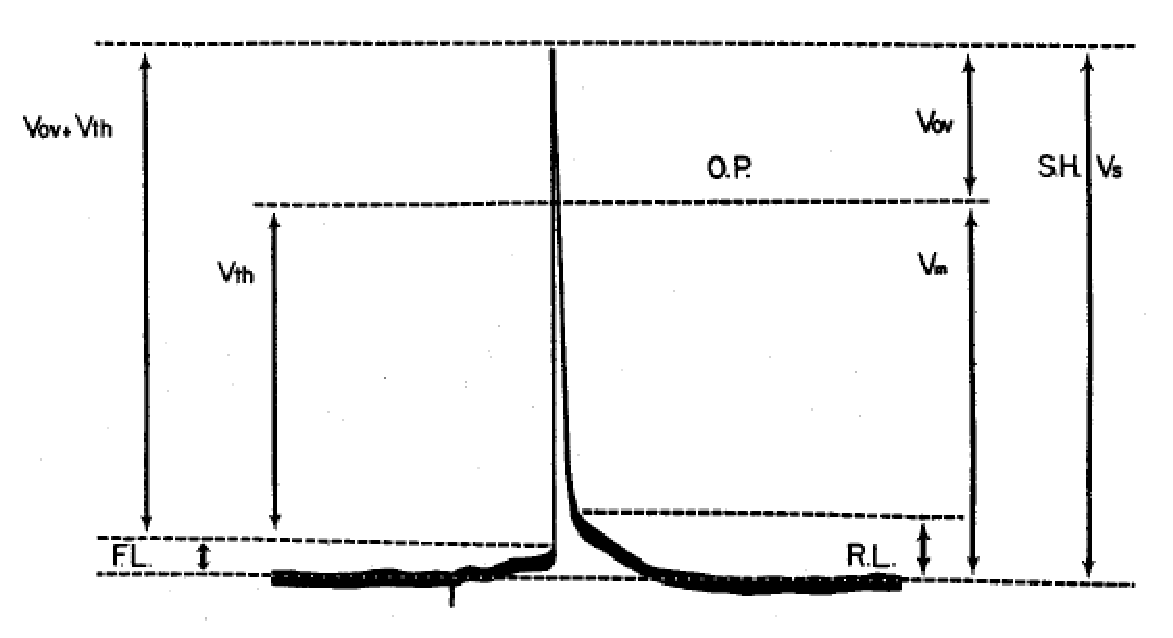
\includegraphics[height=5cm,
    angle=0]{./images/firing_level.eps}}
  \caption{F.L = firing level, S.H. = spike height, R.L. =
    repolarization level, $V_{th}$ = threshold, $V_{ov}$ = overshoot
    voltage, $V_s$ = S.H identified unit, O.P. = outside potential,
    $V_m$ = resting membrane potential}
\label{fig:firing_level}
\end{figure}

Also, with different modes of activations, we observe the similar
spike parameters, as shown in Fig.~\ref{fig:stimulate_mode}.  We will
go in detail in Chap.~\ref{chap:pyramidal-neurons}. 

\begin{figure}[hbt]
  \centerline{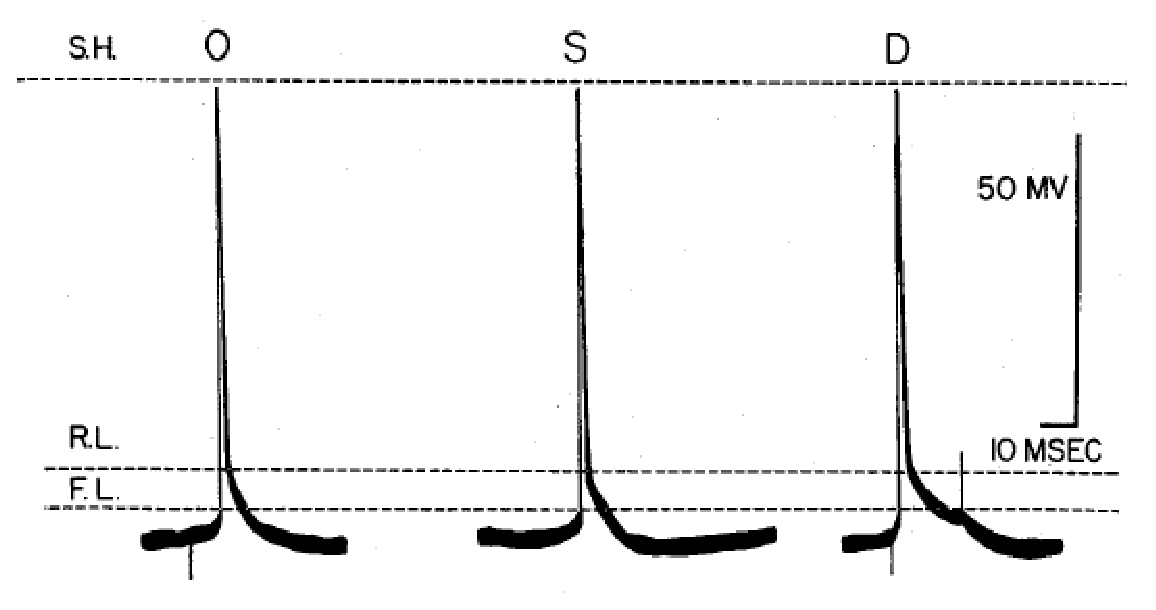
\includegraphics[height=5cm,
    angle=0]{./images/stimulation_mode.eps}}
\caption{O = orthodromically activated, S = spontaneous discharge, D =
activated by direct stimulus delivered through micropipetes, S.H. =
spike height, R.L. = repolarization level, F.L = firing level. }
\label{fig:stimulate_mode}
\end{figure}



\section{Experiment techniques: Interconnection cells}
\label{sec:interc-cells}

The genetically encoded calcium indicators (GCaMP, RCaMP and TNXXL),
voltage sensors (VSFP and Arch), or glutamate sensors (iGluSnFR) enable
the monitoring of neural activity in connectionally-defined neurons and/or
genetically-targeted neurons.




\subsection{Brain slices}
\label{sec:brain-slice}

The widely {\it in vitro} method to study the interconnection between cells is
{\bf brain slice
  techniques}~\cite{rao2004bst, lynch1980ubs, schurr1986bsp, becker2006eub}.
The brain slices can keep the projections and interconnections between cells as
in vivo, yet offer more precisied measurement and more control of environment
variables, as shown in Fig.~\ref{fig:hippocampus}.

The repetitive stimulation at moderate frequency (5 times/sec) produce
a train of AP that last for several seconds afterward. This long-term
potential (LTP) is extremely stable. Experimental results shown that
in cells with high-frequency stimulation, the isolated synaptic
membrane (ISMs) has less phosphate than controlled group. It means
high-frequency stimulation also phosphorylates a specific synaptic
proteins or alter the enzymatic machinery controlling the
phosphorylated state of the protein.
Stimulation also increase intraterminal calcium levels. 

% \begin{figure}[hbt]
%   \centerline{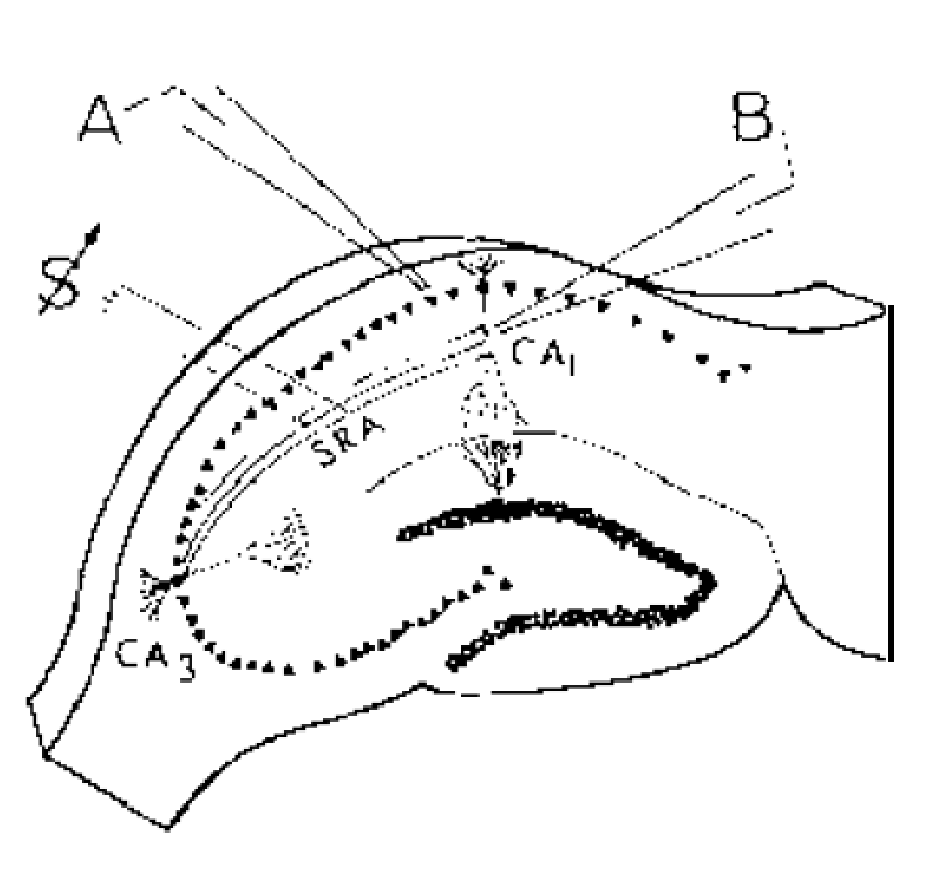
\includegraphics[height=5cm,
%     angle=0]{./images/hippocampus.eps}}
% \caption{A hippocampal slice showing trajectory pathway from CA1 to
%   Schaffer collateral projection (SRA) to CA3}
% \label{fig:hippocampus}
% \end{figure}



% \section{Cable equations}
% \label{sec:cable-equations}

% In the model proposed by Hodgkin-Huxley for squid giant axon, the
% membrane potential was assumed spatial uniformity. {\it In vivo}, the
% intricate branched structure can, however, create spatial gradient in
% the membrane potential. Thus, until the pioneering work of Wilfrid
% Rall (1950s and 1960s), the importance of spatial effects has been
% widely recognized. It is described in the theory of {\bf cable
%   equation}. 

% The theory of flow of electricity in a leaky cable dates back to the
% work of Lord Kelvin in 1855. However, its application to neuronal
% behavior is mainly due to Hodgkin and Ruston (1946) and a series of
% papers by Rall (1957, 1959, 1960, 1969)~\cite{segev1994fdf}

% The cell is viewed as a long cylindrical piece of membrane surrounding
% an interior of cytoplasm (thus called a cable) of unit radius.  Thus,
% the cable can be viewed as one-dimensional. It is said that
% ``everywhere along the cable, the potential depends only on the length
% variable, and not an radial or angular variables''. This is known as
% the {\bf core conductor assumption}.

% The cable is divided into a number of short piece of length $dx$. Each
% piece has isopotential membrane, as shown in
% Fig.~\ref{fig:cable_circuit}. In any cable section, the currents must
% balanced, with only two types of currents: transmembrane current and
% axial current. The transmembrane currents are ionic currents. There
% are two axial currents: intracellular $I_i$ and extracellular $I_e$
% components, both of which are assumed to be linear functions of the
% voltage.
% \begin{figure}[hbt]
%   \centerline{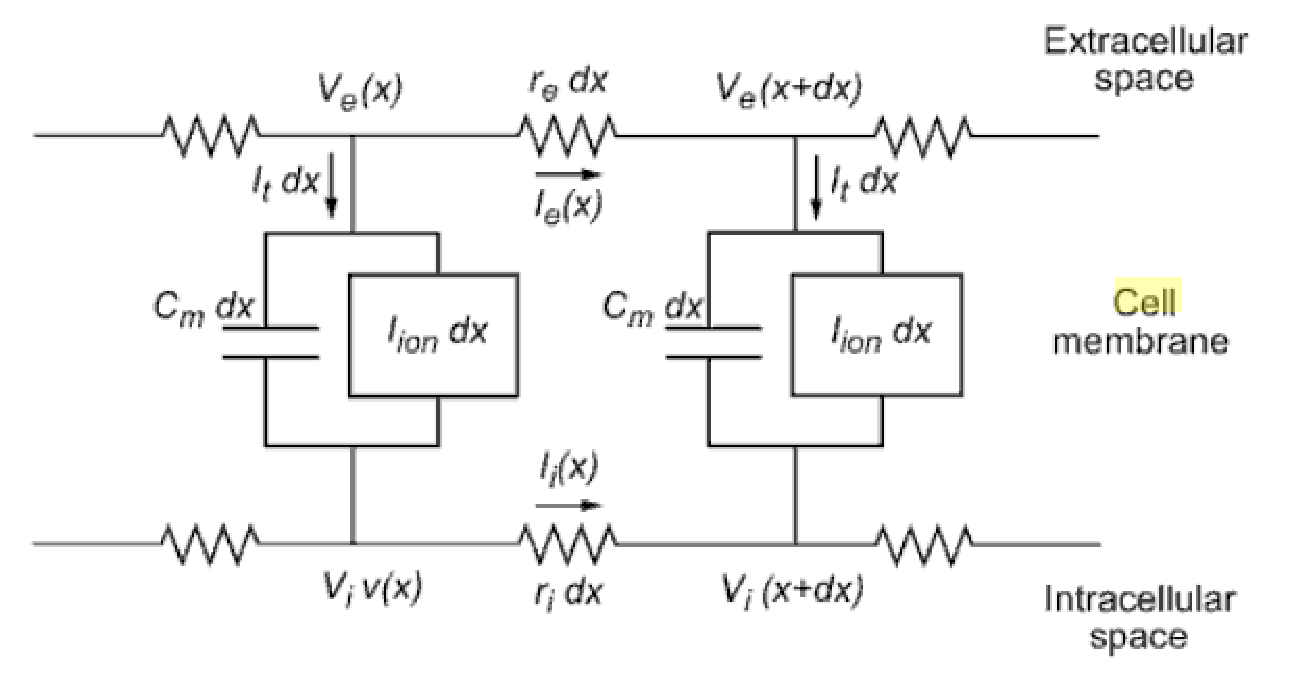
\includegraphics[height=5cm,
%     angle=0]{./images/cable_circuit.eps}}
%   \caption{Schematic diagram of the first discretized cable section of
%     length $dx$}
% \label{fig:cable_circuit}
% \end{figure}

% \begin{equation}
%   \label{eq:421}
%   \begin{split}
%     V_i(x+dx)-V_i(x) &= -r_idx\times I_i(x)\\
%     V_e(x+dx)-V_e(x) &= -r_edx\times I_e(x)\\
%   \end{split}
% \end{equation}
% The minus appears on the right-hand size because of the convention
% that positive current is the flow of positive charges from the left to
% the right (i.e. in the direction of increasing $x$).

% In the limit $dx \rightarrow 0$,
% \begin{equation}
%   \label{eq:422}
%   \begin{split}
%     I_i &= -\frac{1}{r_i}\frac{\partial V_i}{\partial x} \\
%     I_e &= -\frac{1}{r_e}\frac{\partial V_e}{\partial x} \\
%   \end{split}
% \end{equation}
% with $r_i, r_e$ are resistance per unit length (Ohm/mm) of the
% intracellular and extracellular media, respectively.

% If the cable section i-th has the cross section area $A_i$, the the
% resistance per unit length is
% \begin{eqnarray}
%   \label{eq:423}
%   r_i = \frac{R_c}{A_i}
% \end{eqnarray}
% with $R_c$ is the {\bf cytoplasmic resistivity} (Ohm.mm).

% The change in the cytoplasmic current is due to the leak currents
% through the membrane which are the transmembrane current
% \begin{eqnarray}
%   \label{eq:424}
%   I_i(x) - I_i(x+dx) = I_tdx = I_e(x+dx) - I_e(x)
% \end{eqnarray}
% with 
% \begin{eqnarray}
%   \label{eq:425}
%   I_t = p(C_m\frac{\partial V_m}{\partial t} + I_{ion})
% \end{eqnarray}
% with $p$ is the perimeter of the cable (mm$^2$), and $C_m$ is the
% capacitance per unit area of membrane (C/mm$^2$) and $I_{ion}$ has
% unit of current per unit area (A/mm$^2$). $V_m=V_i-V_e$ is the
% membrane potential. 


% In the limit that $dx\rightarrow 0$, 
% \begin{eqnarray}
%   \label{eq:426}
%   I_t = - \frac{\partial I_i}{\partial x} = \frac{\partial I_e}{\partial x} 
% \end{eqnarray}

% At the first cable section, the total axial current is composed of the
% intracellular and extracellular, $I_T = I_i + I_e$; thus using
% eq.~\eqref{eq:422}
% \begin{eqnarray}
%   \label{eq:427}
%   \begin{split}
%       I_T &=  -\frac{1}{r_i}\frac{\partial V_i}{\partial x}
%   -\frac{1}{r_e}\frac{\partial V_e}{\partial x} \\
%    &= -\frac{r_i+r_e}{r_ir_e}\frac{\partial V_i}{\partial x}
%   -\frac{1}{r_e}\frac{\partial V_m}{\partial x} \\
%   \end{split}
% \end{eqnarray}
% with $V_m=V_i-V_e$. Then,
% \begin{eqnarray}
%   \label{eq:428}
%   \frac{1}{r_i}\frac{\partial V_i}{\partial x} =
%   -\frac{1}{r_i+r_e}\frac{\partial V_m}{\partial x} - \frac{r_e}{r_i+r_e}I_T 
% \end{eqnarray}

% Combining eq.~\eqref{eq:422} and eq.~\eqref{eq:426} and
% eq.~\eqref{eq:428}, we have
% \begin{eqnarray}
%   \label{eq:429}
%   I_t = \frac{\partial}{\partial x}\left(
%     \frac{1}{r_i+r_e}\frac{\partial V_m}{\partial x} \right)
% \end{eqnarray}
% as $I_T$ is a constant.

% Combine eq.~\eqref{eq:425}, and eq.~\eqref{eq:429}, we have the {\bf
%   cable equation}
% \begin{eqnarray}
%   \label{eq:430}
%   I_t = p(C_m\frac{\partial V_m}{\partial t} + I_{ion}) =   \frac{\partial}{\partial x}\left(
%     \frac{1}{r_i+r_e}\frac{\partial V_m}{\partial x} \right)
% \end{eqnarray}

% If we applied an external current $I_{app}$ with unit of current per
% unit area across the membrane, then a complete form of the cable
% equation is 
% \begin{eqnarray}
%   \label{eq:431}
%   I_t = p(C_m\frac{\partial V_m}{\partial t} + I_{ion} + I_{app}) =   \frac{\partial}{\partial x}\left(
%     \frac{1}{r_i+r_e}\frac{\partial V_m}{\partial x} \right)
% \end{eqnarray}

% If $R_m$ is the {\bf membrane resistivity}, i.e. resistance of a unit
% square area of the membrane (Ohm.mm$^2$), then for any fixed $V_0$,
% $R_m$ is determined by measuring the change in membrane current when
% $V_m$ is perturbed slightly from $V_0$.
% \begin{eqnarray}
%   \label{eq:432}
%   \frac{1}{R_m} = \frac{dI_{ion}}{dV_m}|_{V_m=V_0}
% \end{eqnarray}

% It is typical to choose $V_0$ as the resting potential to define
% $R_m$. However, if the membrane is an ohmic resistor, then we don't
% need to define $V_0$, as
% \begin{eqnarray}
%   \label{eq:434}
%   R_m = V_m/I_{ion}
% \end{eqnarray}

% Assuming that $r_i, r_e$ are constant, then combining with
% eq.~\eqref{eq:434}, a new form of the cable equation is
% \begin{eqnarray}
%   \label{eq:433}
%   \begin{split}
%     R_mC_m\frac{\partial V_m}{\partial t} + R_mI_{ion} &=
%     \frac{R_m}{p(r_i+r_e)}  \frac{\partial^2V_m}{\partial x^2}\\
%     \tau_m\frac{\partial V_m}{\partial t} + R_mI_{ion} &=
%     \lambda_m^2  \frac{\partial^2V_m}{\partial x^2}\\
%   \end{split}
% \end{eqnarray}
% with $\lambda = \sqrt{\frac{R_m}{p(r_i+r_e)}}$ has the unit of
% distance and thus is called {\bf space constant}; and $\tau_m=R_mC_m$
% has unit of time and thus is called {\bf time constant}.

% If we ignore the extracellular resistance ($r_e=0$), then $\lambda_m =
% \sqrt{\frac{R_m d}{4R_C}}$ with $d$ is the diameter

% \begin{figure}[hbt]
%   \centerline{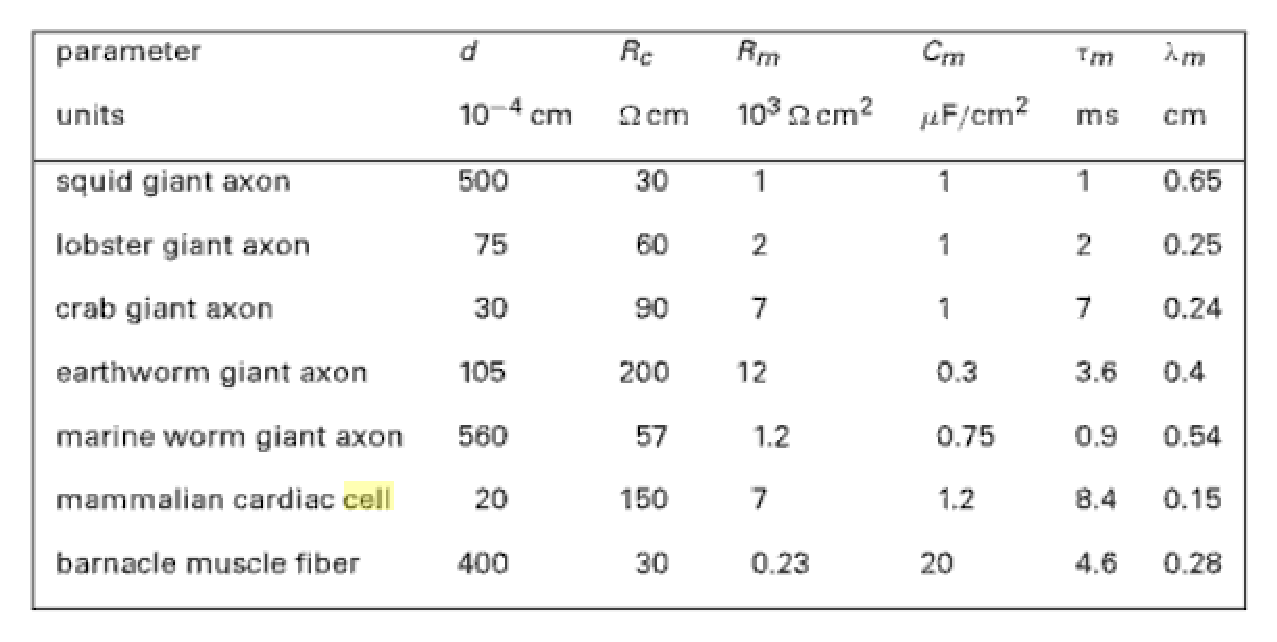
\includegraphics[height=5cm,
%     angle=0]{./images/params_cell.eps}}
% \caption{Typical parameter values for excitable cells}
% \label{fig:param_cell}
% \end{figure}

% To avoid the difference in units, we nondimensionalize the space and
% time by defining new variables $X=x/\lambda_m$ and $T=t/\tau_m$ which
% are both unitless. Then, a unitless equation of the cable equation is
% \begin{eqnarray}
%   \label{eq:436}
%   \frac{\partial V_m}{\partial T}  =
%    \frac{\partial^2V_m}{\partial X^2} + f(V_m,T)
% \end{eqnarray}
% with 
% \begin{eqnarray}
%   \label{eq:437}
%   f(V_m,T) = -I_{ion}R_m
% \end{eqnarray}
% with $f$ is a function of both voltage and time. In simpler cases, $f$
% is a function of $V_m$ only. Typical values for the parameters are shown
% in Fig.~\ref{fig:param_cell}.

\url{http://www.bem.fi/book/02/02.htm}

\url{http://www.tpub.com/content/armymedical/MD0007/MD00070247.htm}

\subsection{Antidromic spikes vs. Orthodromic spike}
\label{sec:antidromic-impulse}

An antidromic impulse in an axon refers to conduction along the axon away from
the axon terminal(s) and towards the soma.
Antidromic activation is often used in a laboratory setting to confirm that a
neuron being recorded from projects to the structure of interest.

Antidromic activation is often induced experimentally by direct electrical
stimulation of a presumed target structure.
Antidromic spikes were evoked by a brief current injection into the
most distal axonal segment


An orthodromic impulse runs along an axon in its normal or anterograde
direction, away from the soma. It refers to the correct direction from the
dendrites to axon terminal. See re-entry (Sect.\ref{sec:re-entry}).

\url{https://en.wikipedia.org/wiki/Antidromic}

